\documentclass[a4paper, 10pt]{article}
\usepackage{../../CEDT-Homework-style}

\usepackage{amsmath}
\allowdisplaybreaks

\setlength{\headheight}{14.49998pt}

\begin{document}
\subject[2110203 - Computer Engineering Mathematics II]
\hwtitle{Signal 1}{}{Week 1}{6733172621 Patthadon Phengpinij}{ChatGPT (for\,\LaTeX\,styling and grammar checking)}


% ================================================================================ %
\section{Representing Signals}
% ================================================================================ %



% ================================================================================ %
%                                    Problem 01                                    %
% ================================================================================ %
\begin{problem}
Sketch the following signals
\end{problem}

% === Problem 1.1. === %

\begin{tosubmit}
\begin{subproblems}
    \item \( x(t) = \sin\frac{\pi}{4} t + 20^\circ \)
\end{subproblems}

\par\noindent\submitsolution
Using Python and Matplotlib to plot the signal \( x(t) = \sin\frac{\pi}{4} t + 20^\circ \):
\begin{codingbox}
import matplotlib.pyplot as plt
import numpy as np

fig = plt.figure()

t = np.arange(-10, 10, 0.01)
x = np.sin(np.pi/4 * t + np.pi/9)

plt.title("Problem 1.1")
plt.plot(t, x)
plt.grid(True)
plt.show()
\end{codingbox}

The plot of the signal is shown below:
\begin{center}
    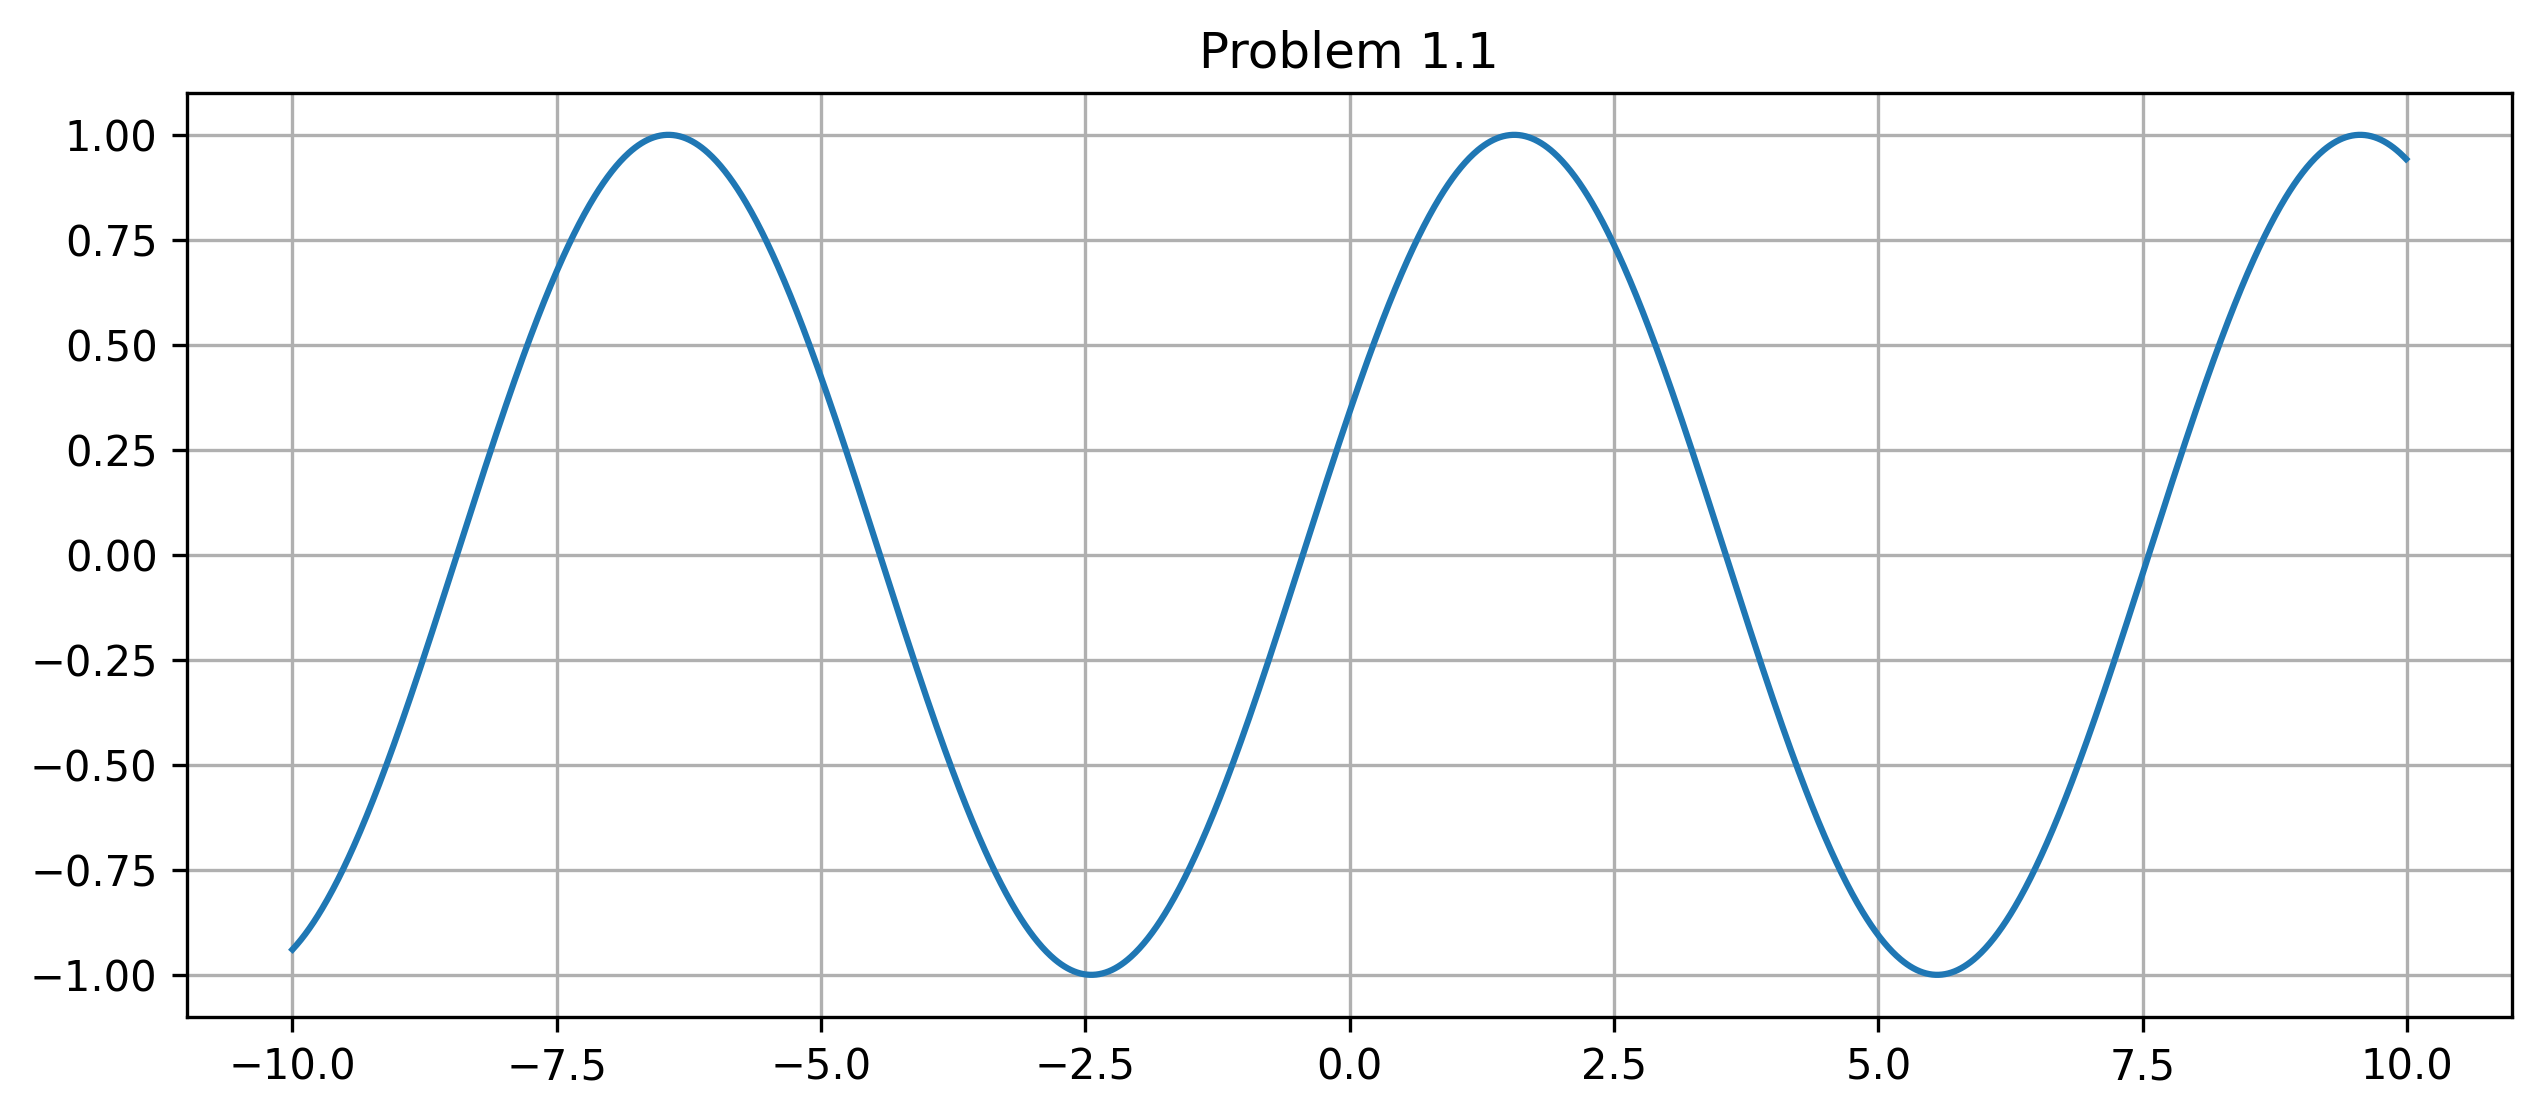
\includegraphics[width=0.8\textwidth]{images/problem_1_1.png}
\end{center}
\end{tosubmit}

% ==================== %

\newpage

% === Problem 1.2. === %
\begin{subproblems}[start=2]
    \item \( x(t) = \begin{cases}
        t + 2, & t \leq 2 \\
        0, & -2 \leq t \leq 2 \\
        t - 2, & t \geq 2
    \end{cases} \)
\end{subproblems}

\begin{solution}
Using Python and Matplotlib to plot the piecewise signal \( x(t) \):
\begin{codingbox}
import matplotlib.pyplot as plt
import numpy as np

fig = plt.figure(figsize=(10, 4))

t = np.arange(-10, 10, 0.01)
x = np.piecewise(t, [t < -2, (t >= -2) & (t < 2), t >= 2], [lambda t: t + 2, 0, lambda t: t - 2])

plt.title("Problem 1.2")
plt.plot(t, x)
plt.grid(True)
plt.show()
\end{codingbox}

The plot of the signal is shown below:
\begin{center}
    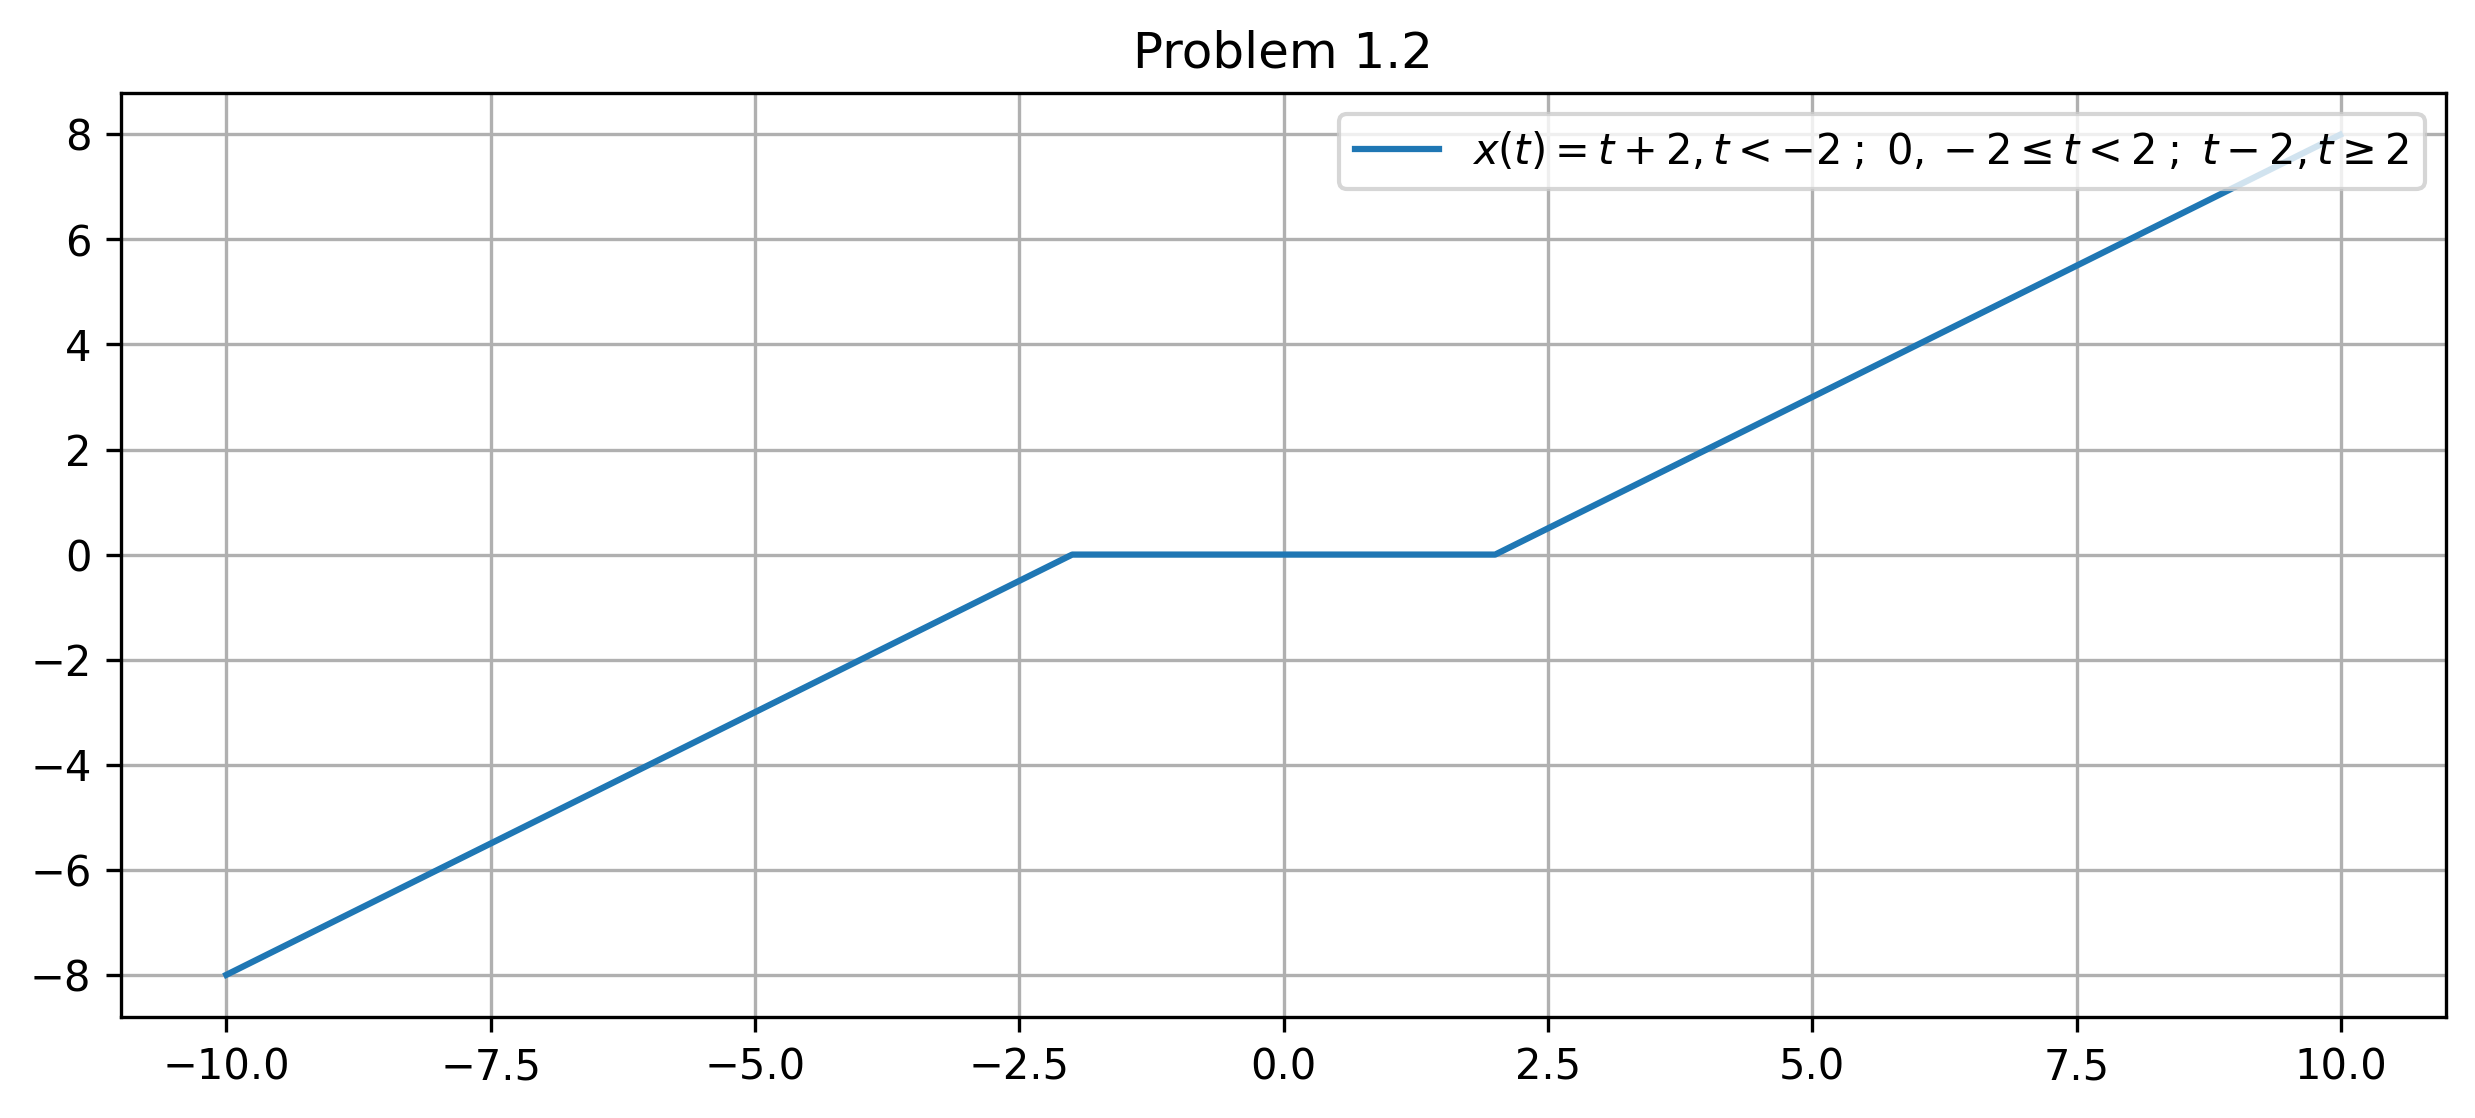
\includegraphics[width=0.8\textwidth]{images/problem_1_2.png}
\end{center}
\end{solution}
% ==================== %

\newpage

% === Problem 1.3. === %
\begin{tosubmit}
\begin{subproblems}[start=3]
    \item \( x(t) = 2e^{-t}, 0 \leq t < 1 \text{ and } x(t + 1) = x(t), \forall t \)
\end{subproblems}

\par\noindent\submitsolution
Using Python and Matplotlib to plot the piecewise signal \( x(t) = 2e^{-t}, 0 \leq t < 1 \text{ and } x(t + 1) = x(t), \forall t \):
\begin{codingbox}
import matplotlib.pyplot as plt
import numpy as np

def x3(t):
    if t >= 1:
        return x3(t - 1)
    if t < 0:
        return x3(t + 1)
    return 2 * (np.e ** (-t))

fig = plt.figure(figsize=(10, 4))

t = np.arange(-10, 10, 0.01)
x3_vectorize = np.vectorize(x3)
x = x3_vectorize(t)

plt.title("Problem 1.3")
plt.plot(t, x)
plt.grid(True)
plt.show()
\end{codingbox}

The plot of the signal is shown below:
\begin{center}
    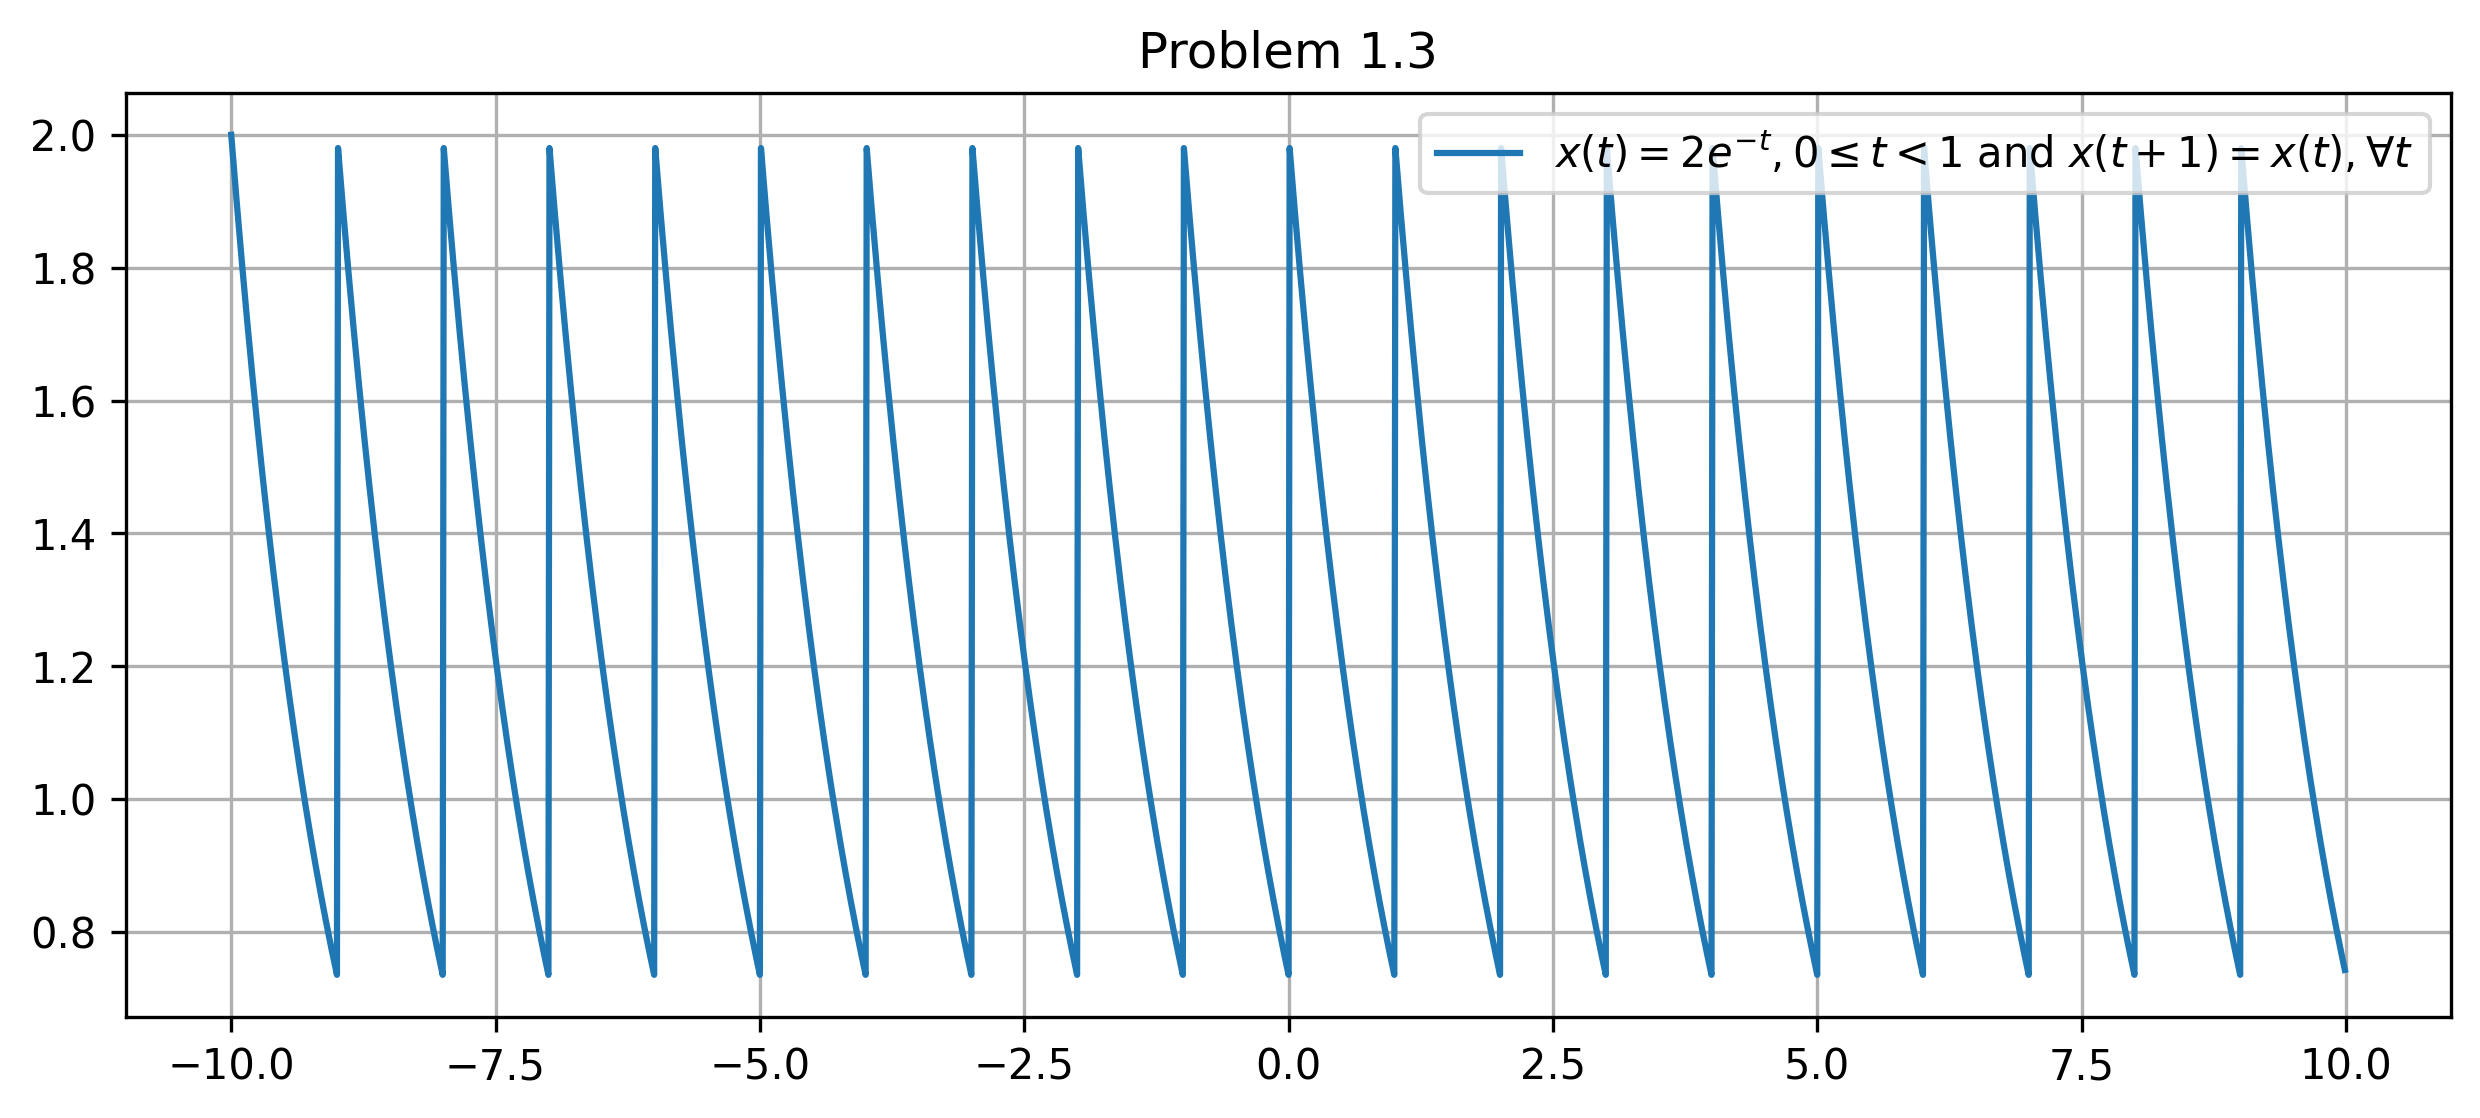
\includegraphics[width=0.8\textwidth]{images/problem_1_3.png}
\end{center}
\end{tosubmit}
% ==================== %

\newpage

% === Problem 1.4. === %
\begin{subproblems}[start=4]
    \item \( x(t) = u(t) + 5u(t - 1) + 2u(t - 2) \)
\end{subproblems}

\begin{solution}
Using Python and Matplotlib to plot the piecewise signal \( x(t) = u(t) + 5u(t - 1) + 2u(t - 2) \):
\begin{codingbox}
import matplotlib.pyplot as plt
import numpy as np

def unit_signal(t):
    return 1.0 if t >= 0 else 0.0

unit_signal_vectorize = np.vectorize(unit_signal)

fig = plt.figure(figsize=(10, 4))

t = np.arange(-6, 6, 0.01)

u1 = unit_signal_vectorize(t)
u2 = unit_signal_vectorize(t - 1)
u3 = unit_signal_vectorize(t - 2)

x = u1 + 5 * u2 - 2 * u3

plt.title("Problem 1.4")
plt.plot(t, x)
plt.grid(True)
plt.show()
\end{codingbox}

The plot of the signal is shown below:
\begin{center}
    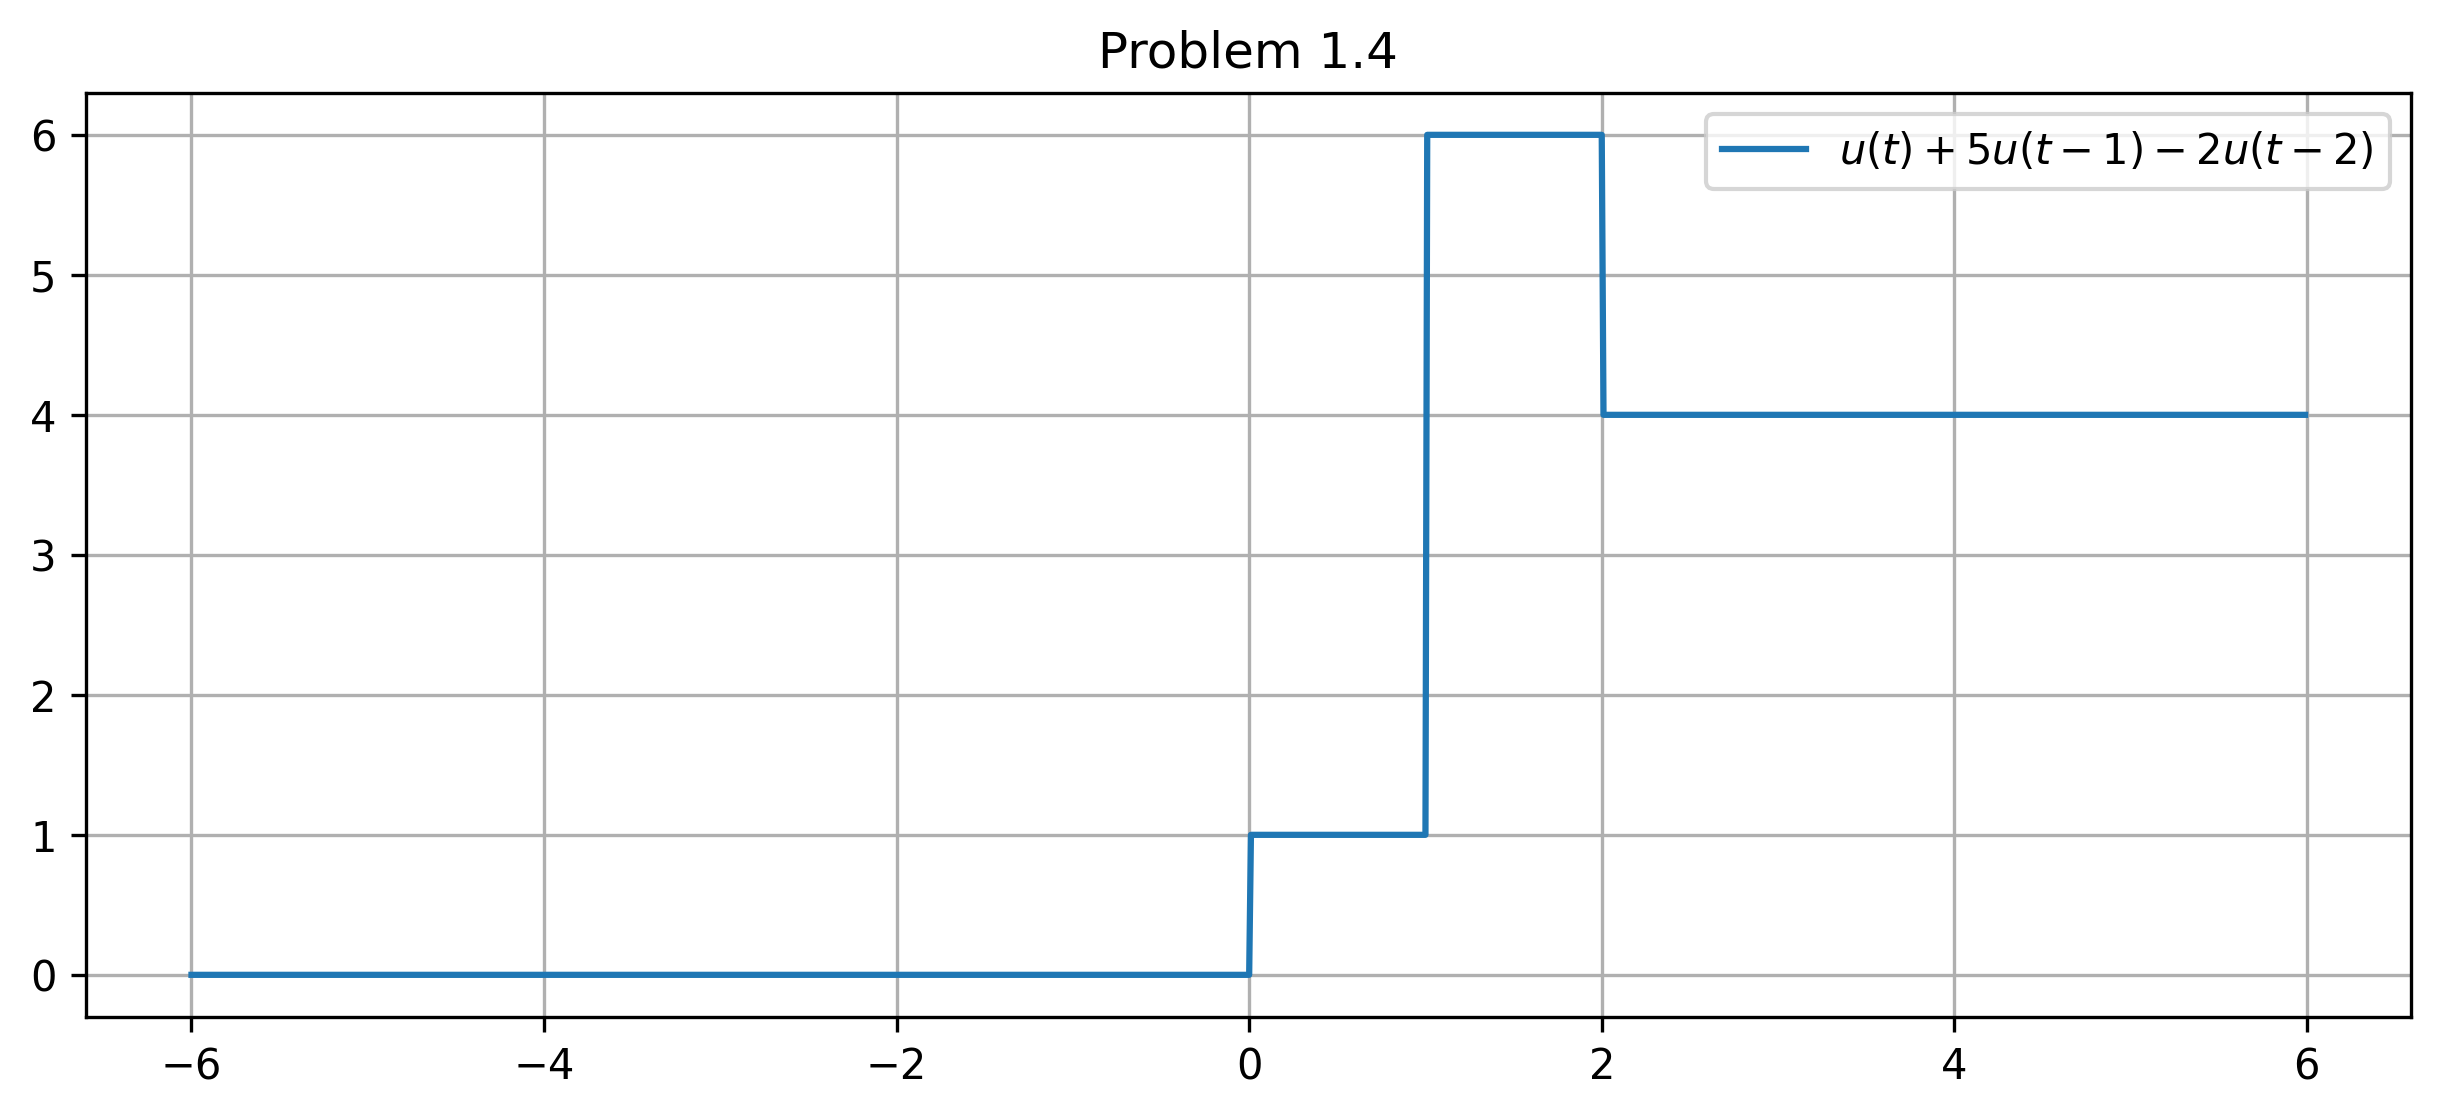
\includegraphics[width=0.8\textwidth]{images/problem_1_4.png}
\end{center}
\end{solution}
% ==================== %

\newpage

% === Problem 1.5. === %
\begin{tosubmit}
\begin{subproblems}[start=5]
    \item \( x(t) = r(t) - r(t - 1) - u(t - 2) \)
\end{subproblems}

\par\noindent\submitsolution
Using Python and Matplotlib to plot the piecewise signal \( x(t) = r(t) - r(t - 1) - u(t - 2) \):
\begin{codingbox}
import matplotlib.pyplot as plt
import numpy as np

def unit_signal(t):
    return 1.0 if t >= 0 else 0.0

def ramp_signal(t):
    return t * unit_signal(t)

unit_signal_vectorize = np.vectorize(unit_signal)
ramp_signal_vectorize = np.vectorize(ramp_signal)

fig = plt.figure(figsize=(10, 4))

t = np.arange(-2, 4, 0.01)

r1 = ramp_signal_vectorize(t)
r2 = ramp_signal_vectorize(t - 1)
u1 = unit_signal_vectorize(t - 2)

x = r1 - r2 - u1

plt.title("Problem 1.5")
plt.plot(t, x)
plt.grid(True)
plt.show()
\end{codingbox}

The plot of the signal is shown below:
\begin{center}
    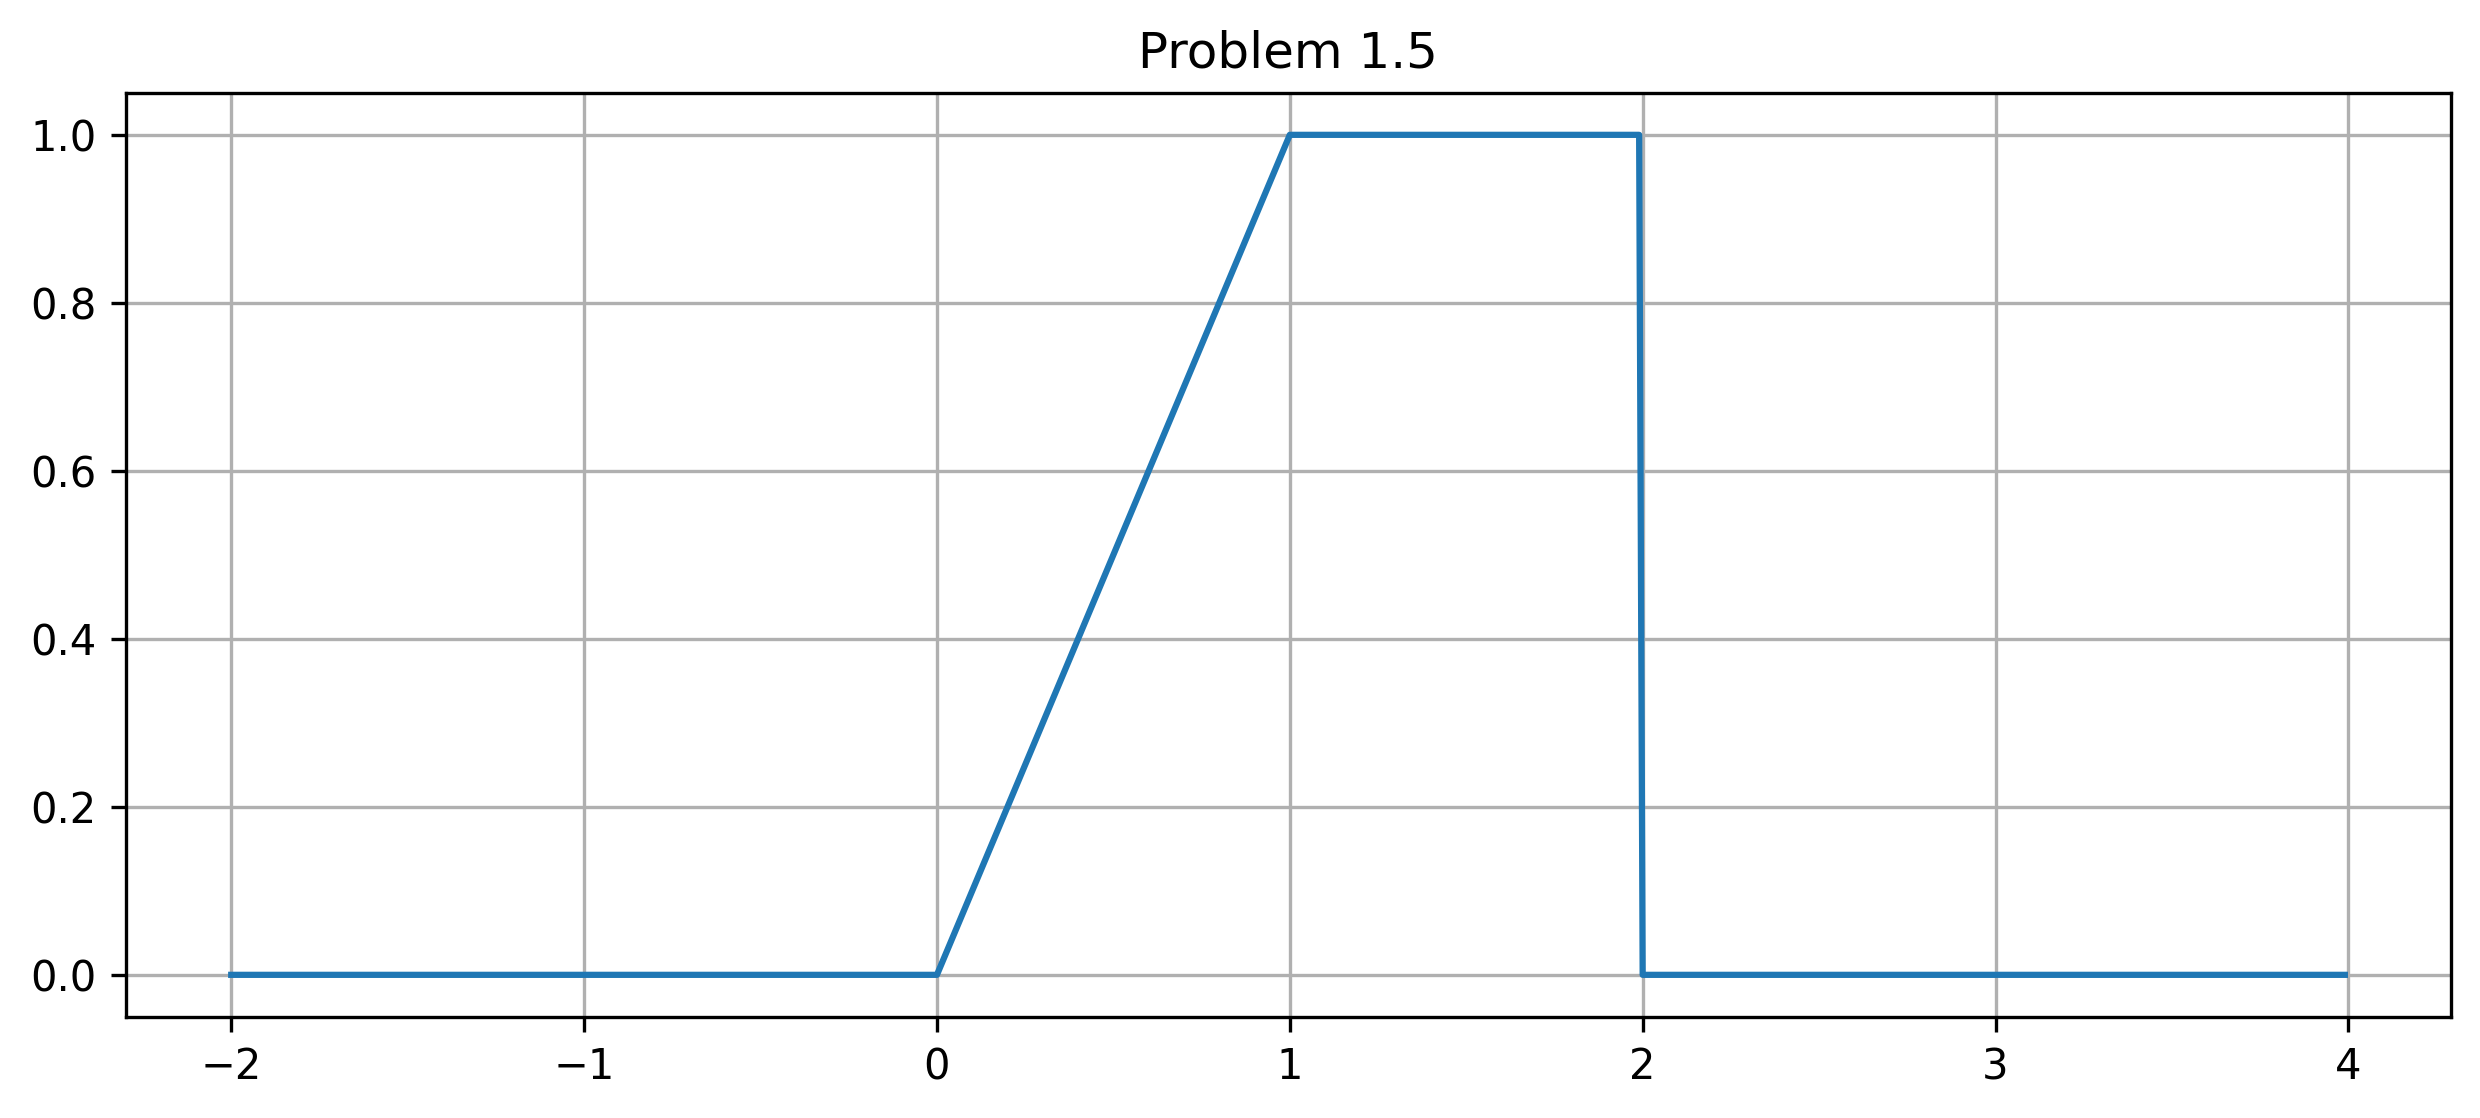
\includegraphics[width=0.8\textwidth]{images/problem_1_5.png}
\end{center}
\end{tosubmit}
% ==================== %

% ================================================================================ %

\newpage

% ================================================================================ %
%                                    Problem 02                                    %
% ================================================================================ %
\begin{problem}
Determine whether each of following signals is periodic, and if so, find its period.
\end{problem}

% === Problem 2.1. === %
\begin{subproblems}
    \item \( x(t) = \sin \paren{ \frac{\pi}{3}t } + \cos \paren{ \frac{8\pi}{3}t } \)
\end{subproblems}

\begin{solution}
Consider each part of the signal separately:
\[
\sin \paren{ \frac{\pi}{3}t } \text{ has a period of } T_1 = \frac{2\pi}{\frac{\pi}{3}} = 6
\]
\[
\cos \paren{ \frac{8\pi}{3}t } \text{ has a period of } T_2 = \frac{2\pi}{\frac{8\pi}{3}} = \frac{3}{4}
\]
Considering the least common multiple of the two periods:
\[
T = \text{lcm}(T_1, T_2) = \text{lcm}(6, \frac{3}{4}) = 6
\]
Thus, the signal \( x(t) = \sin \paren{ \frac{\pi}{3}t } + \cos \paren{ \frac{8\pi}{3}t } \) is periodic with a period of \( T = 6 \).

\vspace{5mm}

By using Python and Matplotlib, we can visualize the periodicity of the signal:
\begin{codingbox}
import matplotlib.pyplot as plt
import numpy as np

fig = plt.figure(figsize=(10, 4))

t = np.arange(-10, 10, 0.01)

x1 = np.sin(np.pi/3 * t)
x2 = np.cos(8*np.pi/3 * t)

x = np.sin(np.pi/3 * t)

plt.title("Problem 2.1")
plt.plot(t, x1 + x2, label="x1(t) + x2(t)")
plt.plot(t, x, label="sinusoidal signal with period 6")
plt.grid(True)
plt.legend(loc="upper right")
plt.show()
\end{codingbox}
The plot of the signal is shown below:
\begin{center}
    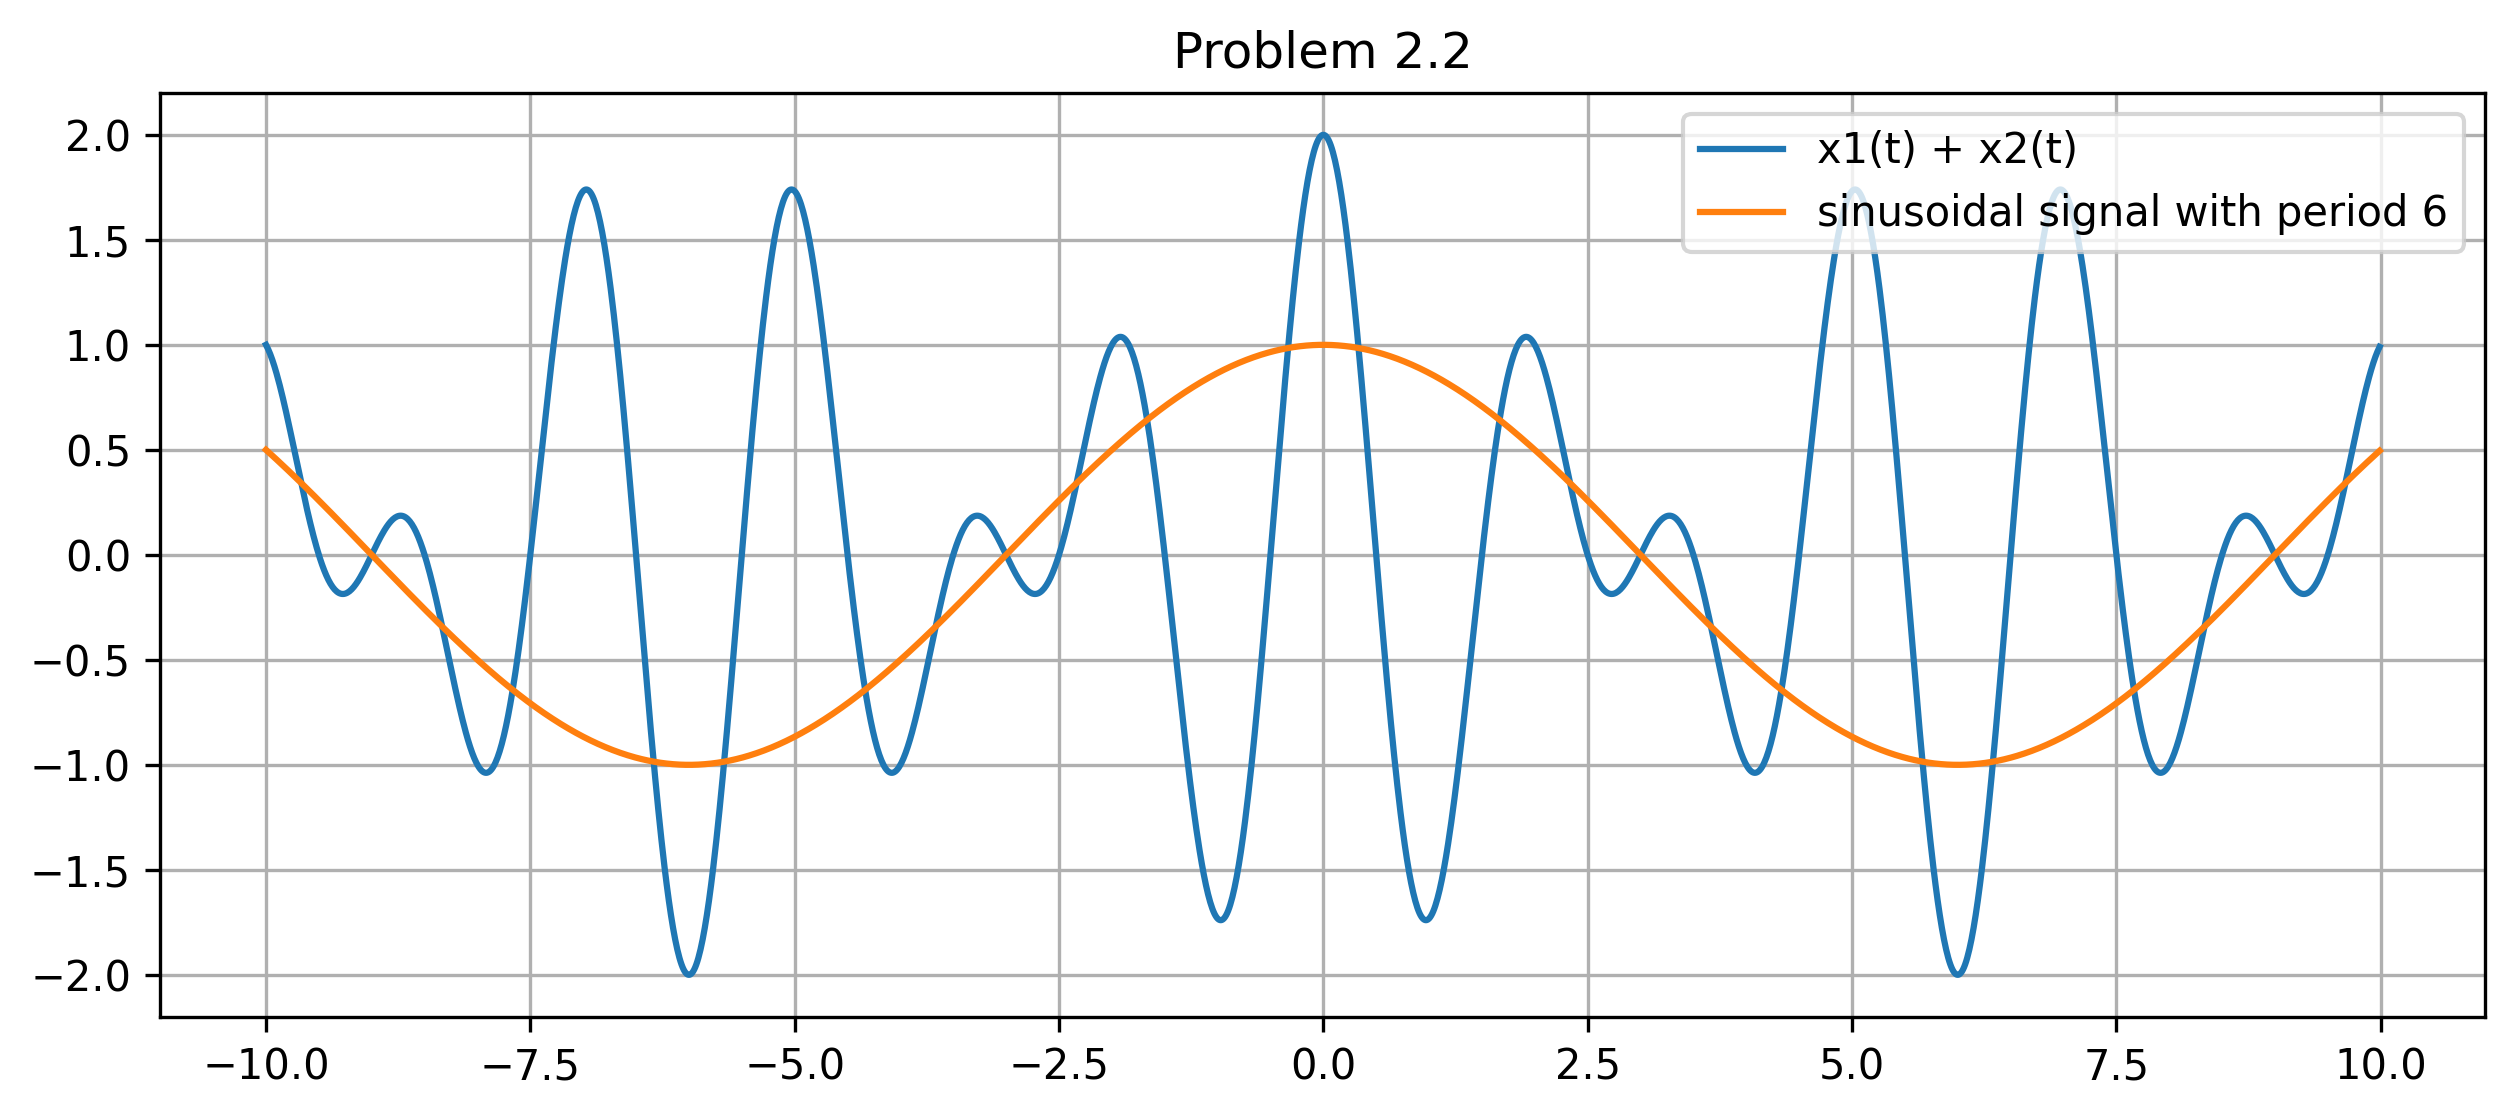
\includegraphics[width=0.8\textwidth]{images/problem_2_1.png}
\end{center}
\end{solution}
% ==================== %

\newpage

% === Problem 2.2. === %
\begin{subproblems}[start=2]
    \item \( x(t) = \exp \paren{ j\frac{7\pi}{6}t } +  \exp \paren{ j\frac{5\pi}{6}t } \)
\end{subproblems}

\begin{solution}
Consider each part of the signal separately:
\[
\exp \paren{ j\frac{7\pi}{6}t } \text{ has a period of } T_1 = \frac{2\pi}{\frac{7\pi}{6}} = \frac{12}{7}
\]
\[
\exp \paren{ j\frac{5\pi}{6}t } \text{ has a period of } T_2 = \frac{2\pi}{\frac{5\pi}{6}} = \frac{12}{5}
\]
Considering the least common multiple of the two periods:
\[
T = \text{lcm}(T_1, T_2) = \text{lcm}\paren{\frac{12}{7}, \frac{12}{5}} = \frac{12}{1} = 12
\]
Thus, the signal \( x(t) = \exp \paren{ j\frac{7\pi}{6}t } +  \exp \paren{ j\frac{5\pi}{6}t } \) is periodic with a period of \( T = 12 \).

\vspace{5mm}

By using Python and Matplotlib, we can visualize the periodicity of the signal:
\begin{codingbox}
import matplotlib.pyplot as plt
import numpy as np

fig = plt.figure(figsize=(10, 4))

t = np.arange(-20, 20, 0.01)

x1 = np.exp(1j * 7*np.pi/6 * t)
x2 = np.exp(1j * 5*np.pi/6 * t)

x = np.exp(1j * np.pi/6 * t)

plt.title("Problem 2.2")
plt.plot(t, x1 + x2, label="x1(t) + x2(t)")
plt.plot(t, x, label="sinusoidal signal with period 12")
plt.grid(True)
plt.legend(loc="upper right")
plt.show()
\end{codingbox}
The plot of the signal is shown below:
\begin{center}
    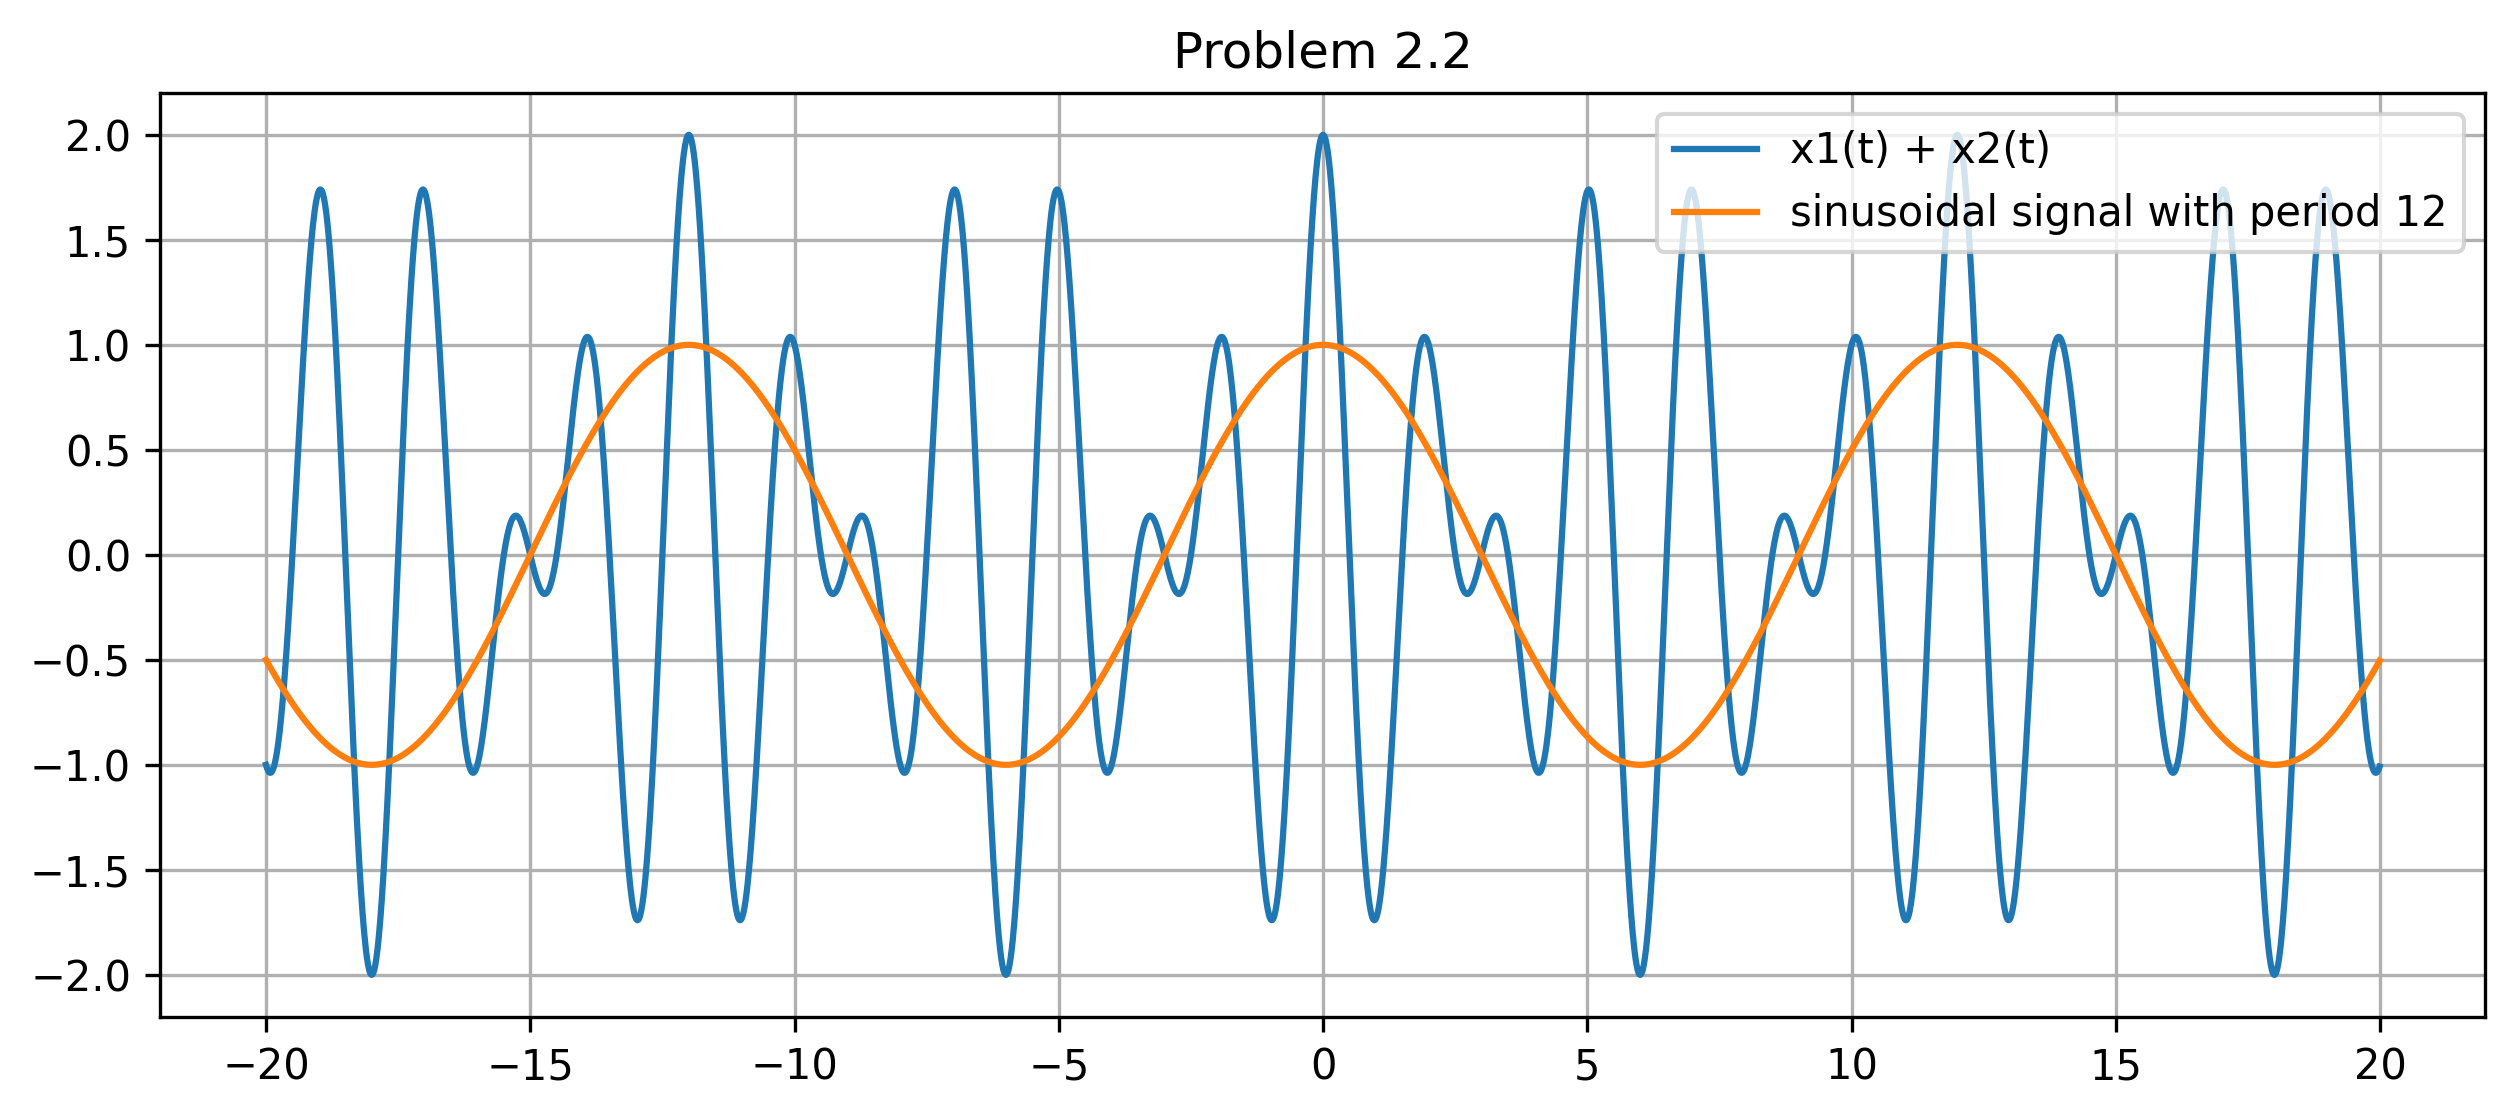
\includegraphics[width=0.8\textwidth]{images/problem_2_2.png}
\end{center}
\end{solution}
% ==================== %

\newpage

% === Problem 2.3. === %
\begin{subproblems}[start=3]
    \item \( x(t) = \exp \paren{ j\frac{7\pi}{6}t } +  \exp \paren{ \frac{5\pi}{6}t } \)
\end{subproblems}

\begin{solution}
Consider each part of the signal separately:
\[
\exp \paren{ j\frac{7\pi}{6}t } \text{ has a period of } T_1 = \frac{2\pi}{\frac{7\pi}{6}} = \frac{12}{7}
\]
\[
\exp \paren{ \frac{5\pi}{6}t } \text{ has no period since it is not a sinusoidal function. (non-periodic signal) }
\]
Thus, the signal \( x(t) = \exp \paren{ j\frac{7\pi}{6}t } +  \exp \paren{ \frac{5\pi}{6}t } \) is non-periodic since one part of the signal is non-periodic.

\vspace{5mm}

By using Python and Matplotlib, we can visualize the signal:
\begin{codingbox}
import matplotlib.pyplot as plt
import numpy as np

fig = plt.figure(figsize=(10, 4))

t = np.arange(-5, 5, 0.01)

x1 = np.exp(1j * 7*np.pi/6 * t)
x2 = np.exp(5*np.pi/6 * t)

plt.title("Problem 2.3")
plt.plot(t, x1 + x2, label="x1(t) + x2(t)")
plt.grid(True)
plt.legend(loc="upper right")
plt.show()
\end{codingbox}
The plot of the signal is shown below:
\begin{center}
    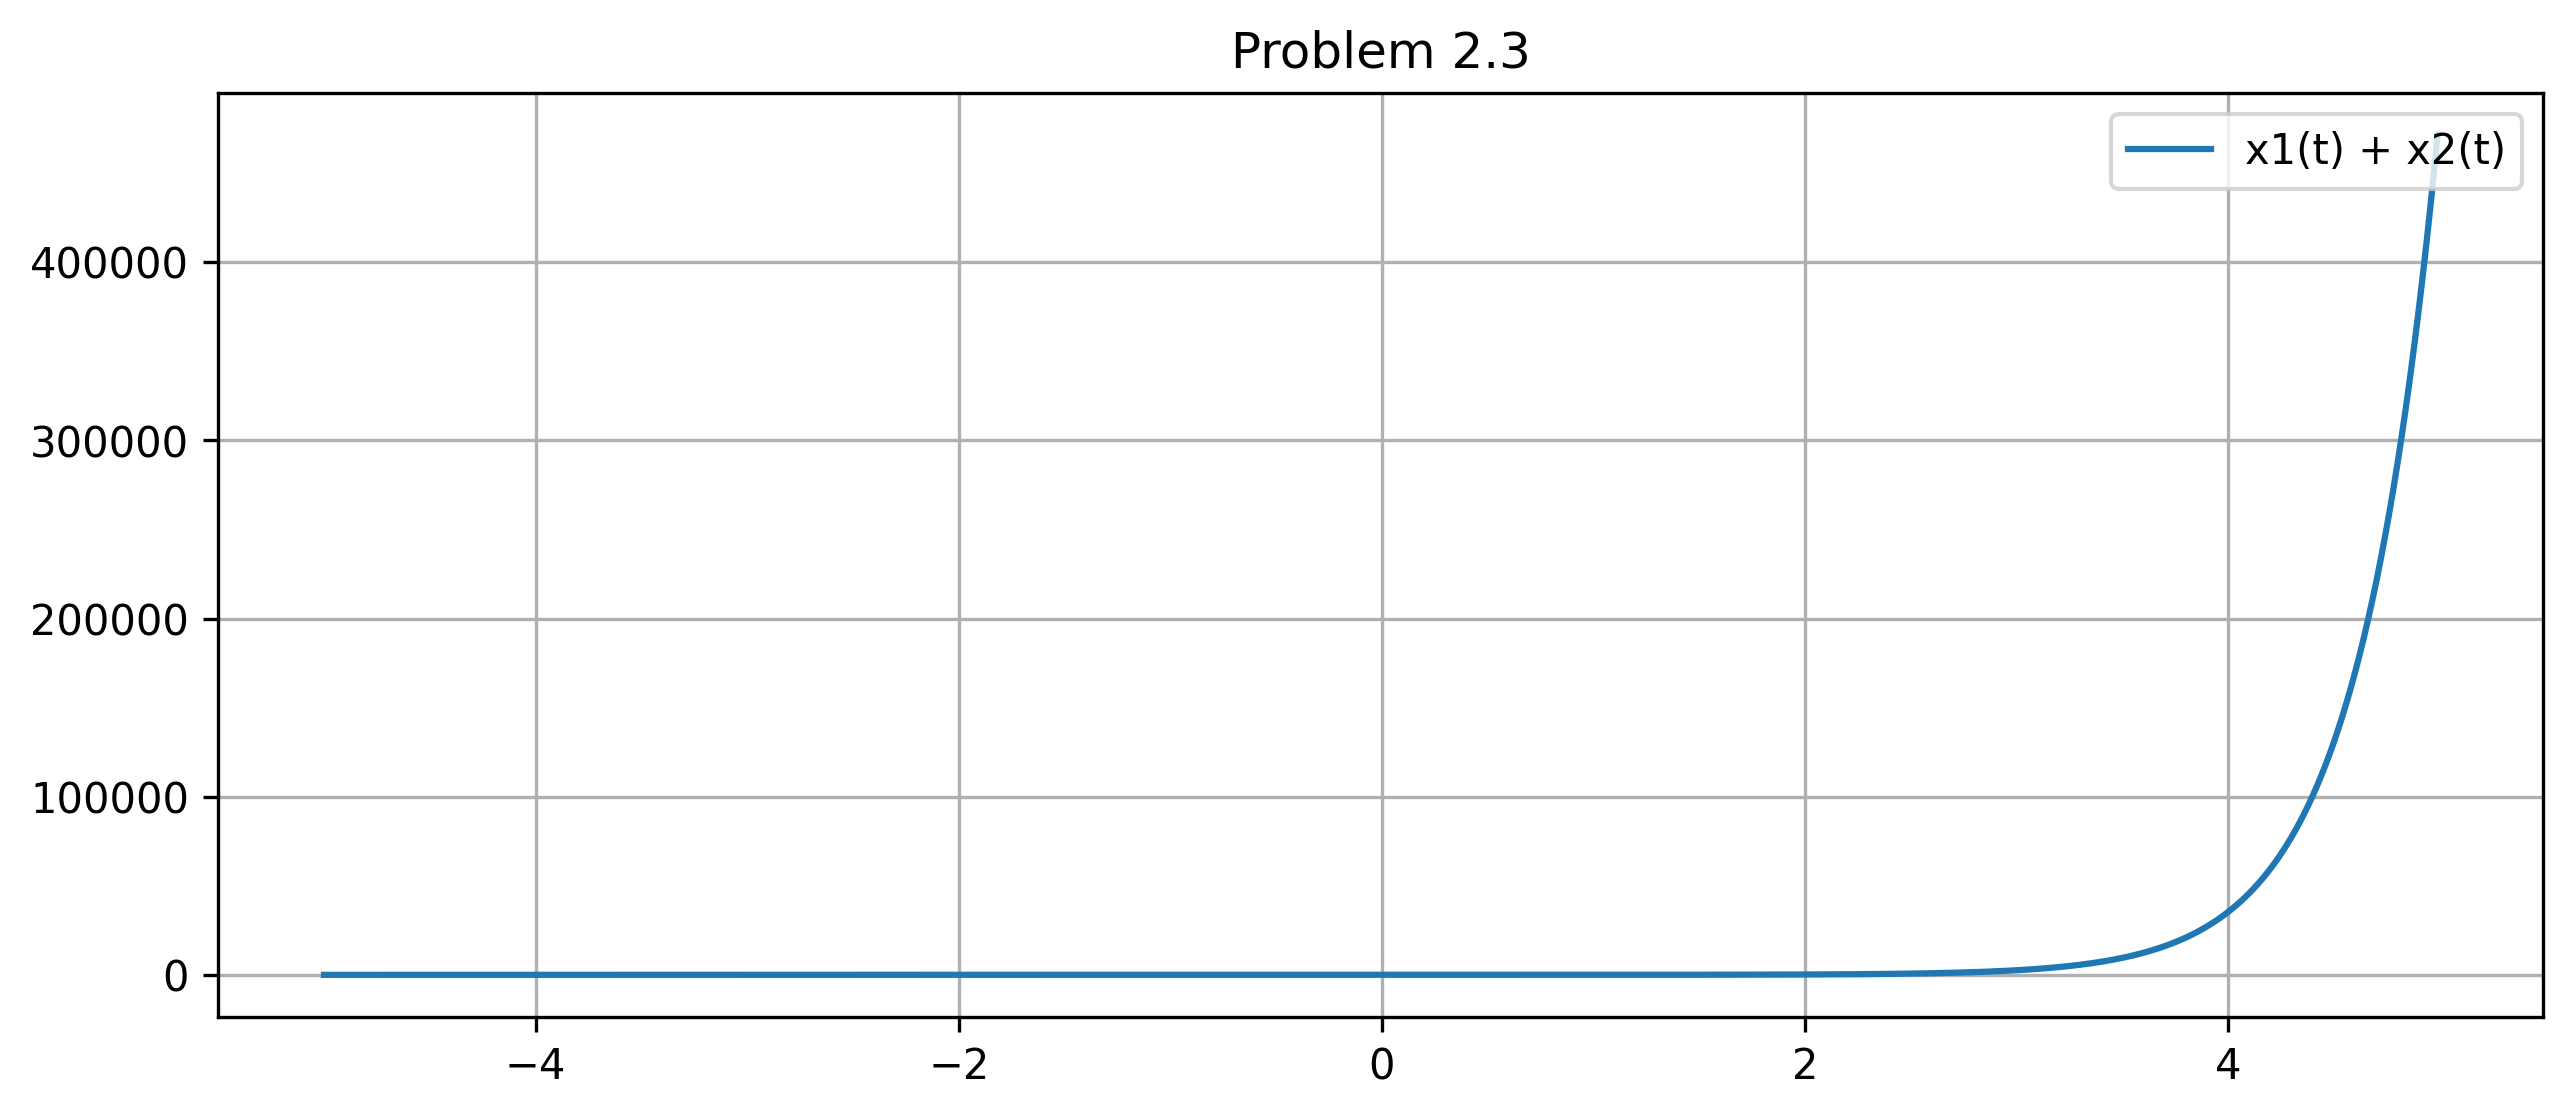
\includegraphics[width=0.8\textwidth]{images/problem_2_3.png}
\end{center}
\end{solution}
% ==================== %
% ================================================================================ %

\newpage

% ================================================================================ %
%                                    Problem 03                                    %
% ================================================================================ %
\begin{problem}
Determine whether the following signals are power or energy signals or neither. Justify your answers
\end{problem}

% === Problem 3.1. === %
\begin{subproblems}
    \item \( x(t) = A\sin( t ), -\infty < t < \infty \)
\end{subproblems}

\begin{solution}
Consider the energy of the signal:
\begin{align*}
    E &= \lim_{N \to \infty} \int_{-N}^{N} |x(t)|^2 dt \\
    &= \lim_{N \to \infty} \int_{-N}^{N} |A\sin(t)|^2 dt \\
    &= \lim_{N \to \infty} A^2 \int_{-N}^{N} \sin^2(t) dt \\
    &= \lim_{N \to \infty} A^2 \int_{-N}^{N} \frac{1 - \cos(2t)}{2} dt \\
    &= \lim_{N \to \infty} \frac{A^2}{2} \sqbracket{ t - \frac{\sin(2t)}{2} }_{-N}^{N} \\
    &= \lim_{N \to \infty} \frac{A^2}{2} \paren{ N - (-N) } \\
    &= \lim_{N \to \infty} A^2 N \\
    E &= \infty
\end{align*}
The integral diverges, so the energy is infinite.

\vspace{5mm}

Now, consider the power of the signal:
\begin{align*}
    P &= \lim_{N \to \infty} \frac{1}{2N} \int_{-N}^{N} |x(t)|^2 dt \\
    &= \lim_{N \to \infty} \frac{1}{2N} A^2 N \\
    P &= \frac{A^2}{2}
\end{align*}
The integral converges to a finite value, so the power is finite.

\vspace{2mm}

Thus, the signal \( x(t) = A\sin( t ) \) is \textbf{a power signal} with power \( P = \frac{A^2}{2} \).

\vspace{2mm}

By using Python and Matplotlib, we can visualize the signal:
\begin{codingbox}
import matplotlib.pyplot as plt
import numpy as np

fig = plt.figure(figsize=(10, 4))

t = np.arange(-10, 10, 0.01)
x = np.sin(t)

plt.title("Problem 3.1")
plt.plot(t, x, label="x(t), A = 1")
plt.grid(True)
plt.legend(loc="upper right")
plt.show()
\end{codingbox}

\newpage

The plot of the signal is shown below:
\begin{center}
    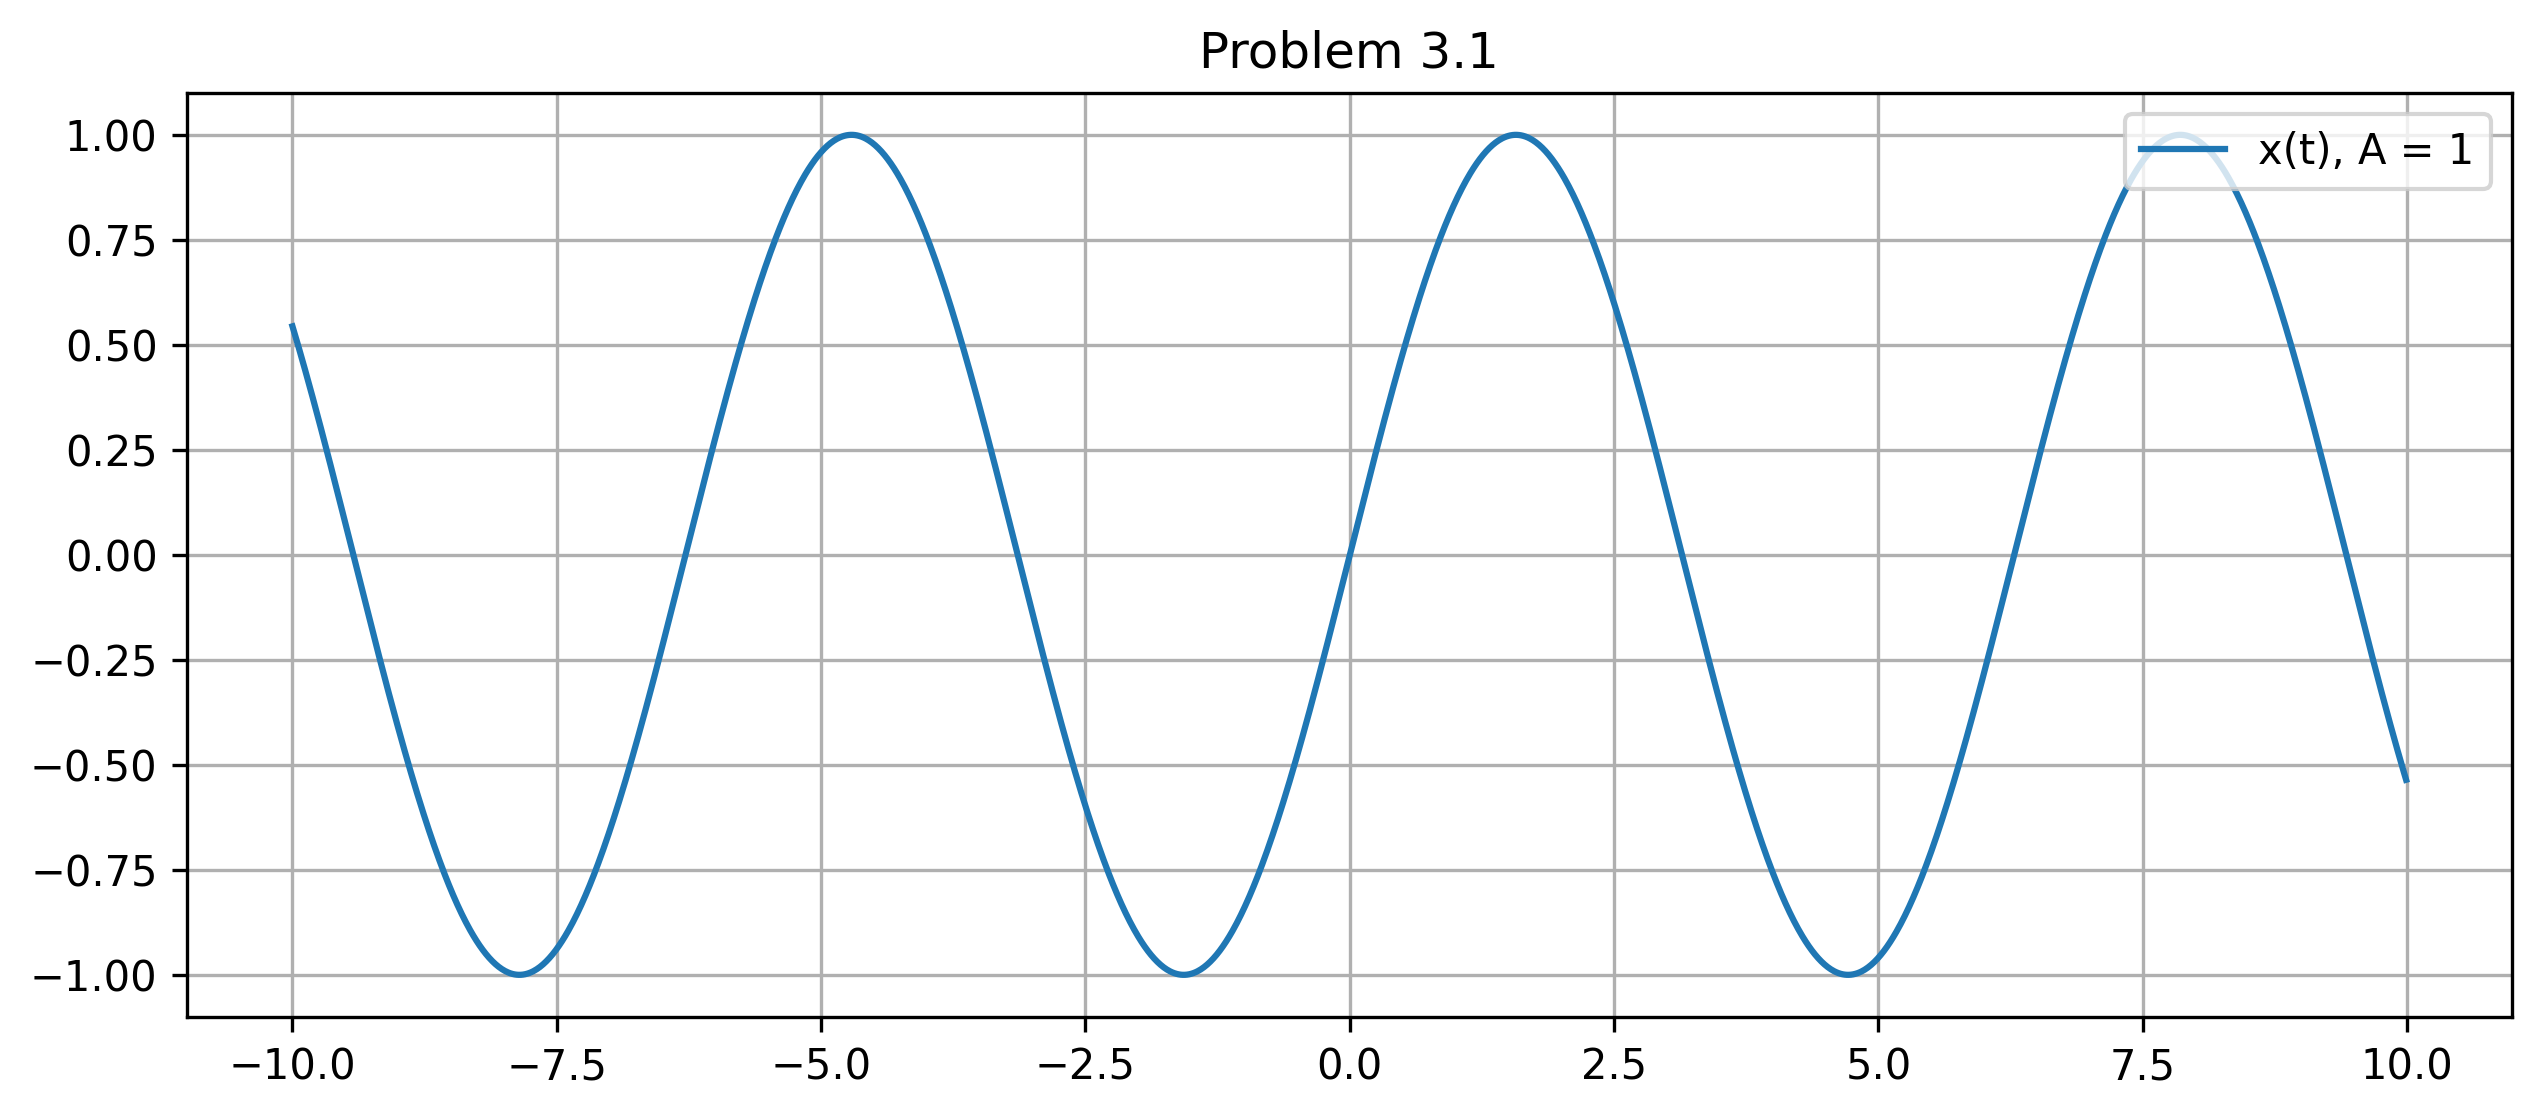
\includegraphics[width=0.8\textwidth]{images/problem_3_1.png}
\end{center}
\end{solution}
% ==================== %


% === Problem 3.2. === %
\begin{subproblems}[start=2]
    \item \( x(t) = A(u(t-a) - u(t+a)), \, a > 0 \)
\end{subproblems}

\begin{solution}
Consider the energy of the signal:
\begin{align*}
    E &= \lim_{N \to \infty} \int_{-N}^{N} |x(t)|^2 dt \\
    &= \lim_{N \to \infty} \int_{-N}^{N} |A(u(t-a) - u(t+a))|^2 dt \\
    &= \lim_{N \to \infty} A^2 \int_{-N}^{N} |u(t-a) - u(t+a)|^2 dt \\
    &= \lim_{N \to \infty} A^2 \int_{-N}^{N} (u(t-a) - u(t+a))^2 dt \\
    &= \lim_{N \to \infty} A^2 \int_{-N}^{N} (u(t+a) - u(t-a)) dt \\
    &= \lim_{N \to \infty} A^2 \int_{-a}^{a} 1 dt \\
    &= \lim_{N \to \infty} A^2 (a - (-a)) \\
    E &= 2aA^2
\end{align*}
The integral converges to a finite value, so the energy is finite.

\vspace{5mm}

Now, consider the power of the signal:
\begin{align*}
    P &= \lim_{N \to \infty} \frac{1}{2N} \int_{-N}^{N} |x(t)|^2 dt \\
    &= \lim_{N \to \infty} \frac{1}{2N} 2aA^2 \\
    P &= 0
\end{align*}
The integral converges to 0, so the power is 0.

\vspace{2mm}

Thus, the signal \( x(t) = A(u(t-a) - u(t+a)) \) is \textbf{a energy signal} with energy \( E = 2aA^2 \).

\vspace{2mm}

By using Python and Matplotlib, we can visualize the signal:
\begin{codingbox}
import matplotlib.pyplot as plt
import numpy as np

def unit_signal(t):
    return 1.0 if t >= 0 else 0.0

unit_signal_vectorize = np.vectorize(unit_signal)

fig = plt.figure(figsize=(10, 4))

t = np.arange(-4, 4, 0.01)
x = unit_signal_vectorize(t - 1) - unit_signal_vectorize(t + 1)

plt.title("Problem 3.2")
plt.plot(t, x, label="x(t), a = 1, A = 1")
plt.grid(True)
plt.legend(loc="upper right")
plt.show()
\end{codingbox}

\newpage

The plot of the signal is shown below:
\begin{center}
    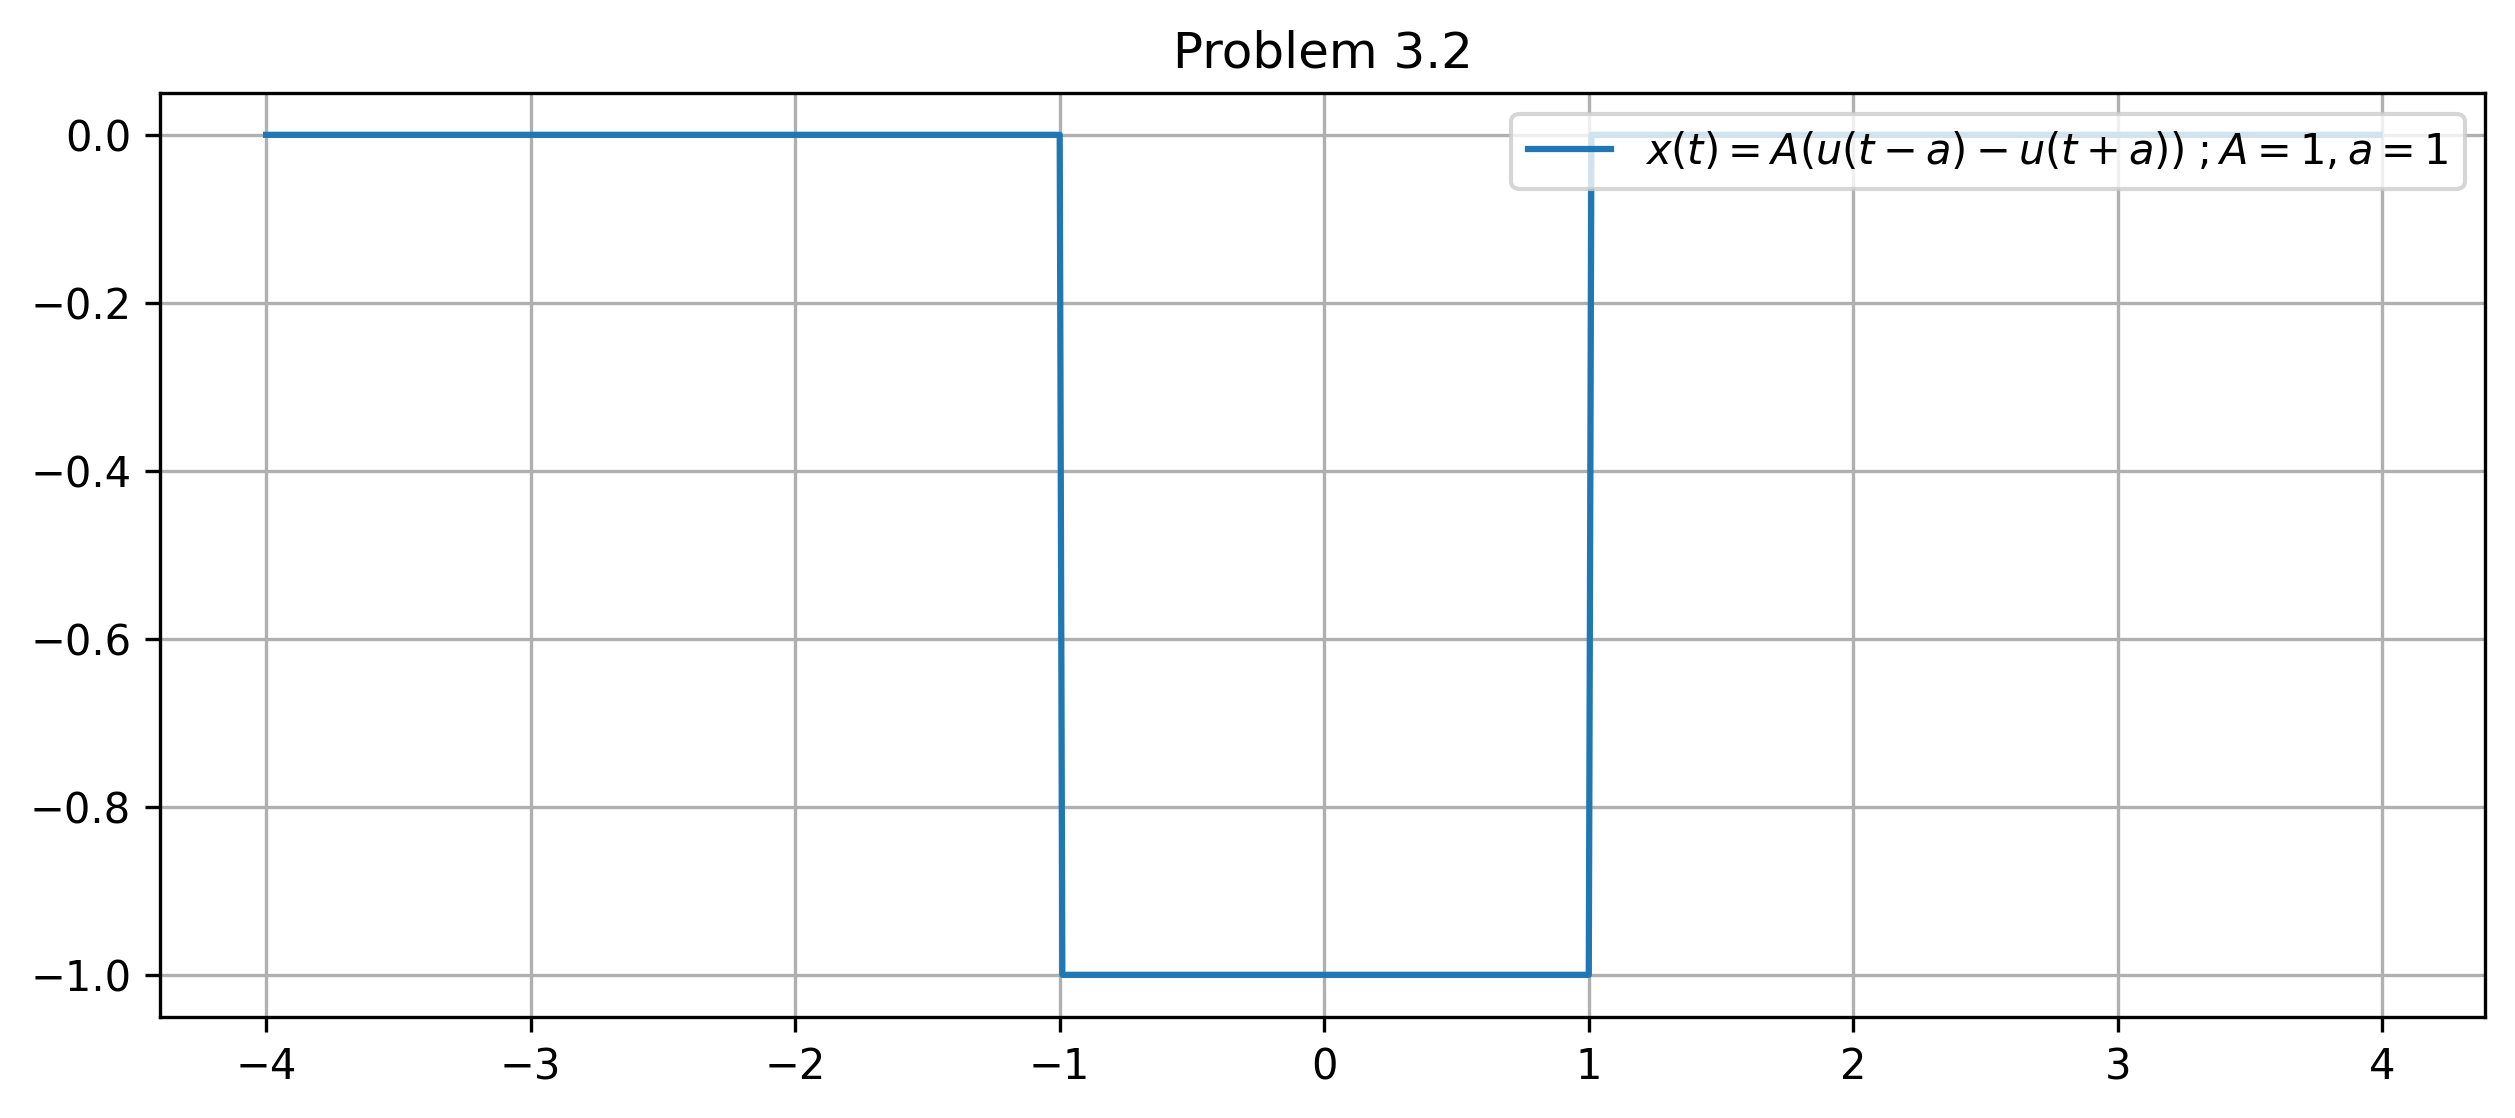
\includegraphics[width=0.8\textwidth]{images/problem_3_2.png}
\end{center}
\end{solution}
% ==================== %


% === Problem 3.3. === %
\begin{subproblems}[start=3]
    \item \( x(t) = \exp(-at)u(t), \,  a > 0 \)
\end{subproblems}

\begin{solution}
Consider the energy of the signal:
\begin{align*}
    E &= \lim_{N \to \infty} \int_{-N}^{N} |x(t)|^2 dt \\
    &= \lim_{N \to \infty} \int_{-N}^{N} |\exp(-at)u(t)|^2 dt \\
    &= \lim_{N \to \infty} \int_{0}^{N} |\exp(-at)|^2 dt \\
    &= \lim_{N \to \infty} \int_{0}^{N} \exp(-2at) dt \\
    &= \lim_{N \to \infty} \sqbracket{ -\frac{1}{2a} \exp(-2at) }_{0}^{N} \\
    &= \lim_{N \to \infty} \paren{ -\frac{1}{2a} \exp(-2aN) + \frac{1}{2a} } \\
    E &= \frac{1}{2a}
\end{align*}
The integral converges to a finite value, so the energy is finite.

\vspace{5mm}

Now, consider the power of the signal:
\begin{align*}
    P &= \lim_{N \to \infty} \frac{1}{2N} \int_{-N}^{N} |x(t)|^2 dt \\
    &= \lim_{N \to \infty} \frac{1}{2N} \frac{1}{2a} \\
    P &= 0
\end{align*}
The integral converges to 0, so the power is 0.

\vspace{2mm}

Thus, the signal \( x(t) = \exp(-at)u(t), \,  a > 0 \) is \textbf{a energy signal} with energy \( E = \frac{1}{2a} \).

\vspace{2mm}

By using Python and Matplotlib, we can visualize the signal:
\begin{codingbox}
import matplotlib.pyplot as plt
import numpy as np

def unit_signal(t):
    return 1.0 if t >= 0 else 0.0

unit_signal_vectorize = np.vectorize(unit_signal)

fig = plt.figure(figsize=(10, 4))

t = np.arange(-8, 8, 0.01)
x = np.exp(-t) * unit_signal_vectorize(t)

plt.title("Problem 3.3")
plt.plot(t, x, label="x(t), a = 1")
plt.grid(True)
plt.legend(loc="upper right")
plt.show()
\end{codingbox}

\newpage

The plot of the signal is shown below:
\begin{center}
    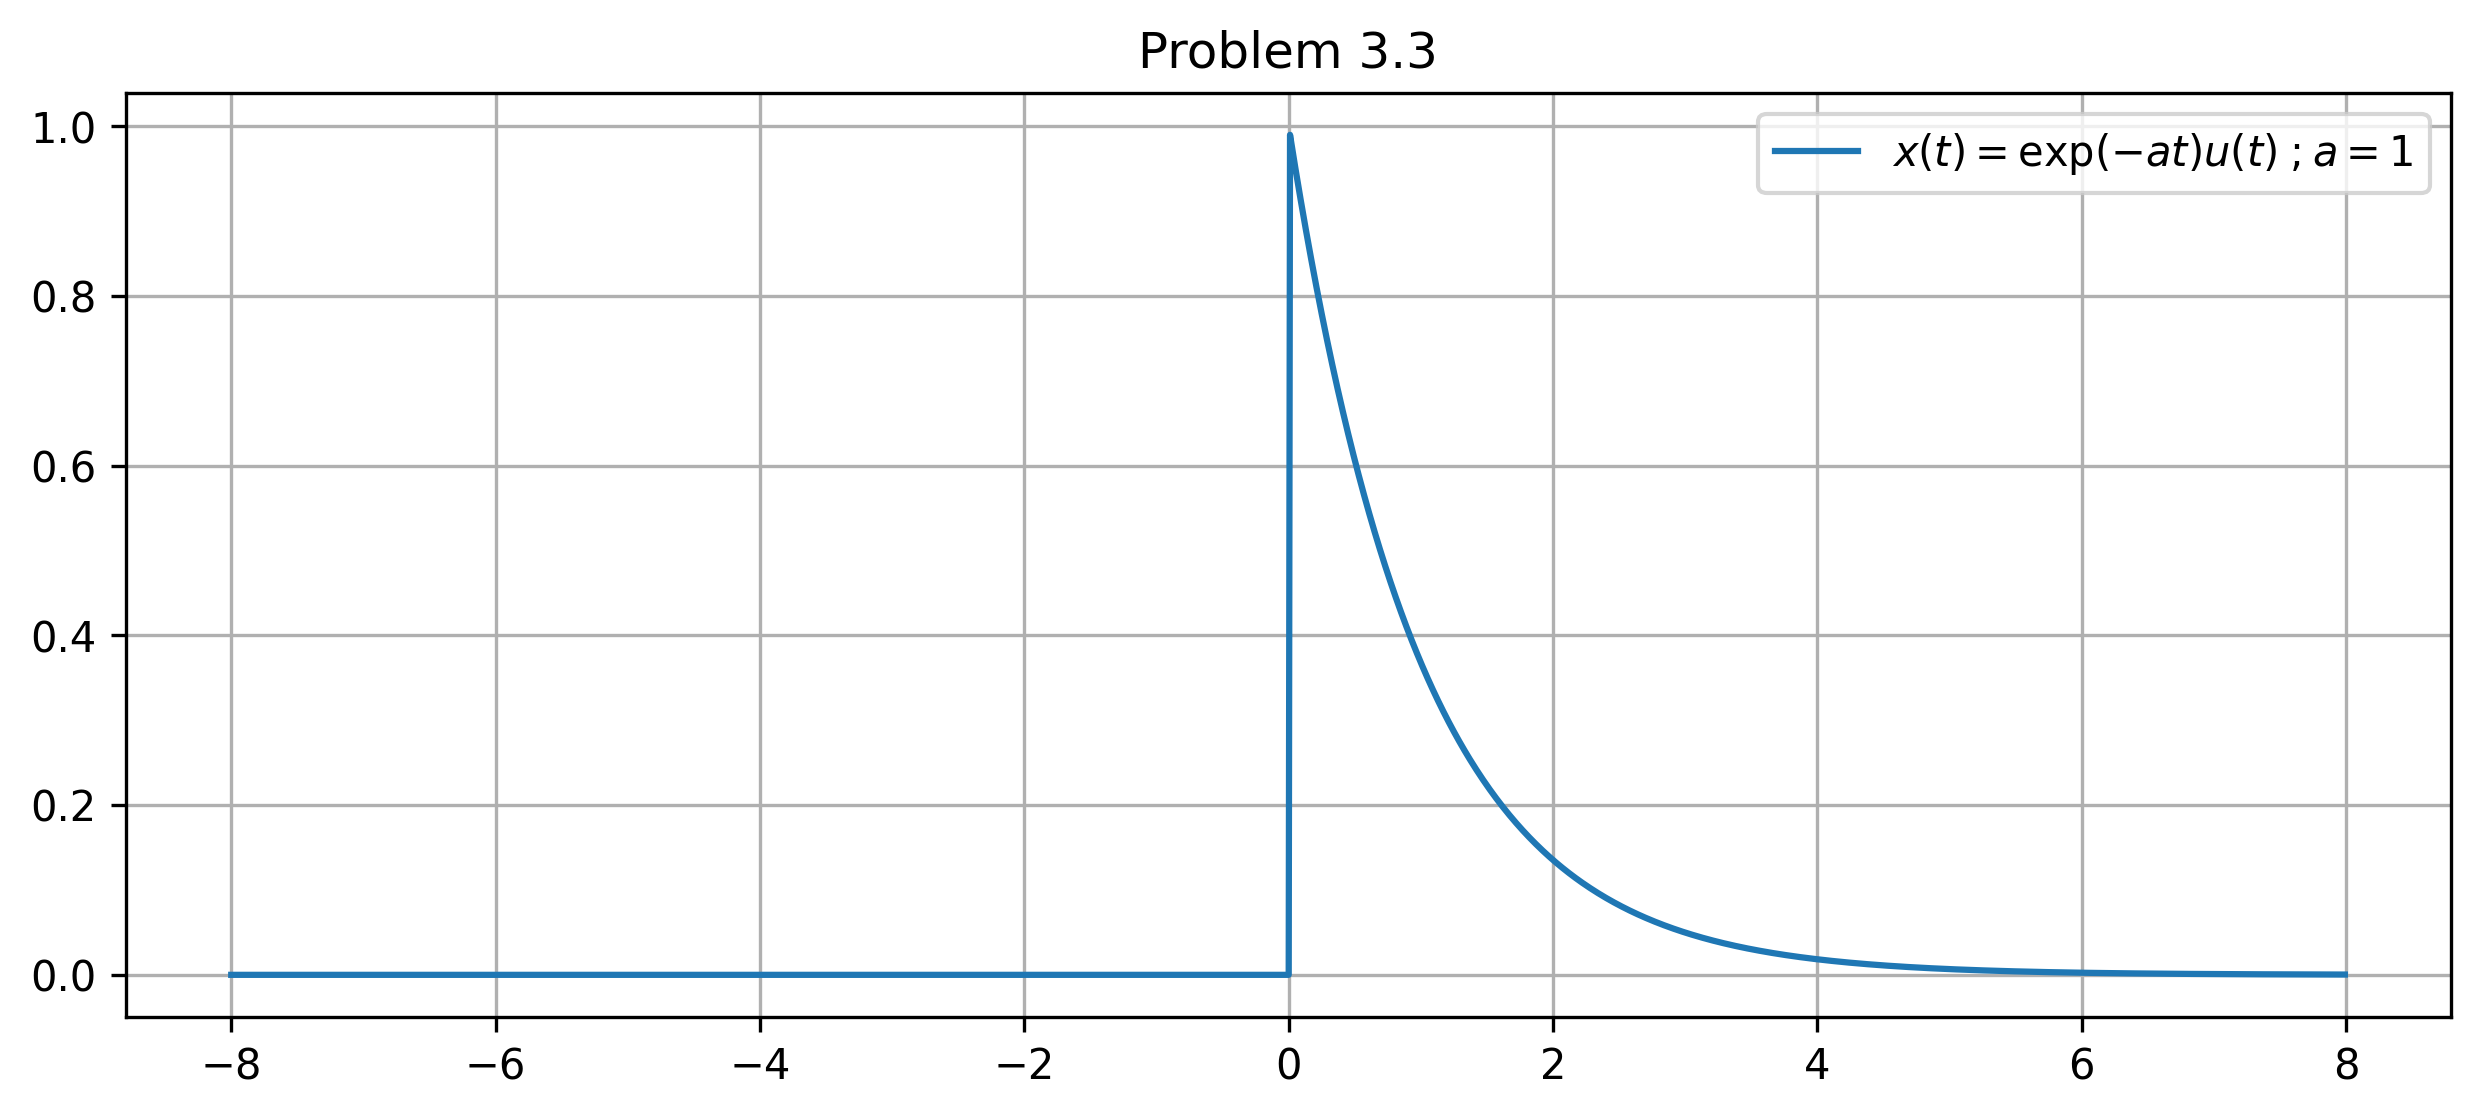
\includegraphics[width=0.8\textwidth]{images/problem_3_3.png}
\end{center}
\end{solution}
% ==================== %

\newpage

% === Problem 3.4. === %
\begin{subproblems}[start=4]
    \item \( x(t) = A\exp(bt)u(t), \, b > 0 \)
\end{subproblems}

\begin{solution}
Consider the energy of the signal:
\begin{align*}
    E &= \lim_{N \to \infty} \int_{-N}^{N} |x(t)|^2 dt \\
    &= \lim_{N \to \infty} \int_{-N}^{N} |A\exp(bt)u(t)|^2 dt \\
    &= \lim_{N \to \infty} \int_{0}^{N} |A\exp(bt)|^2 dt \\
    &= \lim_{N \to \infty} \int_{0}^{N} A^2\exp(2bt) dt \\
    &= \lim_{N \to \infty} A^2 \sqbracket{ \frac{1}{2b} \exp(2bt) }_{0}^{N} \\
    &= \lim_{N \to \infty} A^2 \paren{ \frac{1}{2b} \exp(2bN) - \frac{1}{2b} } \\
    E &= \infty
\end{align*}
The integral diverges, so the energy is infinite.

\vspace{5mm}

Now, consider the power of the signal:
\begin{align*}
    P &= \lim_{N \to \infty} \frac{1}{2N} \int_{-N}^{N} |x(t)|^2 dt \\
    &= \lim_{N \to \infty} \frac{1}{2N} A^2 \paren{ \frac{1}{2b} \exp(2bN) - \frac{1}{2b} } \\
    P &= \infty
\end{align*}
The integral diverges, so the power is infinite.

\vspace{2mm}

Thus, the signal \( x(t) = A\exp(bt)u(t), \,  b > 0 \) is \textbf{neither a energy nor a power signal}.

\vspace{2mm}

By using Python and Matplotlib, we can visualize the signal:
\begin{codingbox}
import matplotlib.pyplot as plt
import numpy as np

def unit_signal(t):
    return 1.0 if t >= 0 else 0.0

unit_signal_vectorize = np.vectorize(unit_signal)

fig = plt.figure(figsize=(10, 4))

t = np.arange(-4, 6, 0.01)
x = np.exp(t) * unit_signal_vectorize(t)

plt.title("Problem 3.4")
plt.plot(t, x, label="x(t), A = 1, b = 1")
plt.grid(True)
plt.legend(loc="upper right")
plt.show()
\end{codingbox}

\newpage

The plot of the signal is shown below:
\begin{center}
    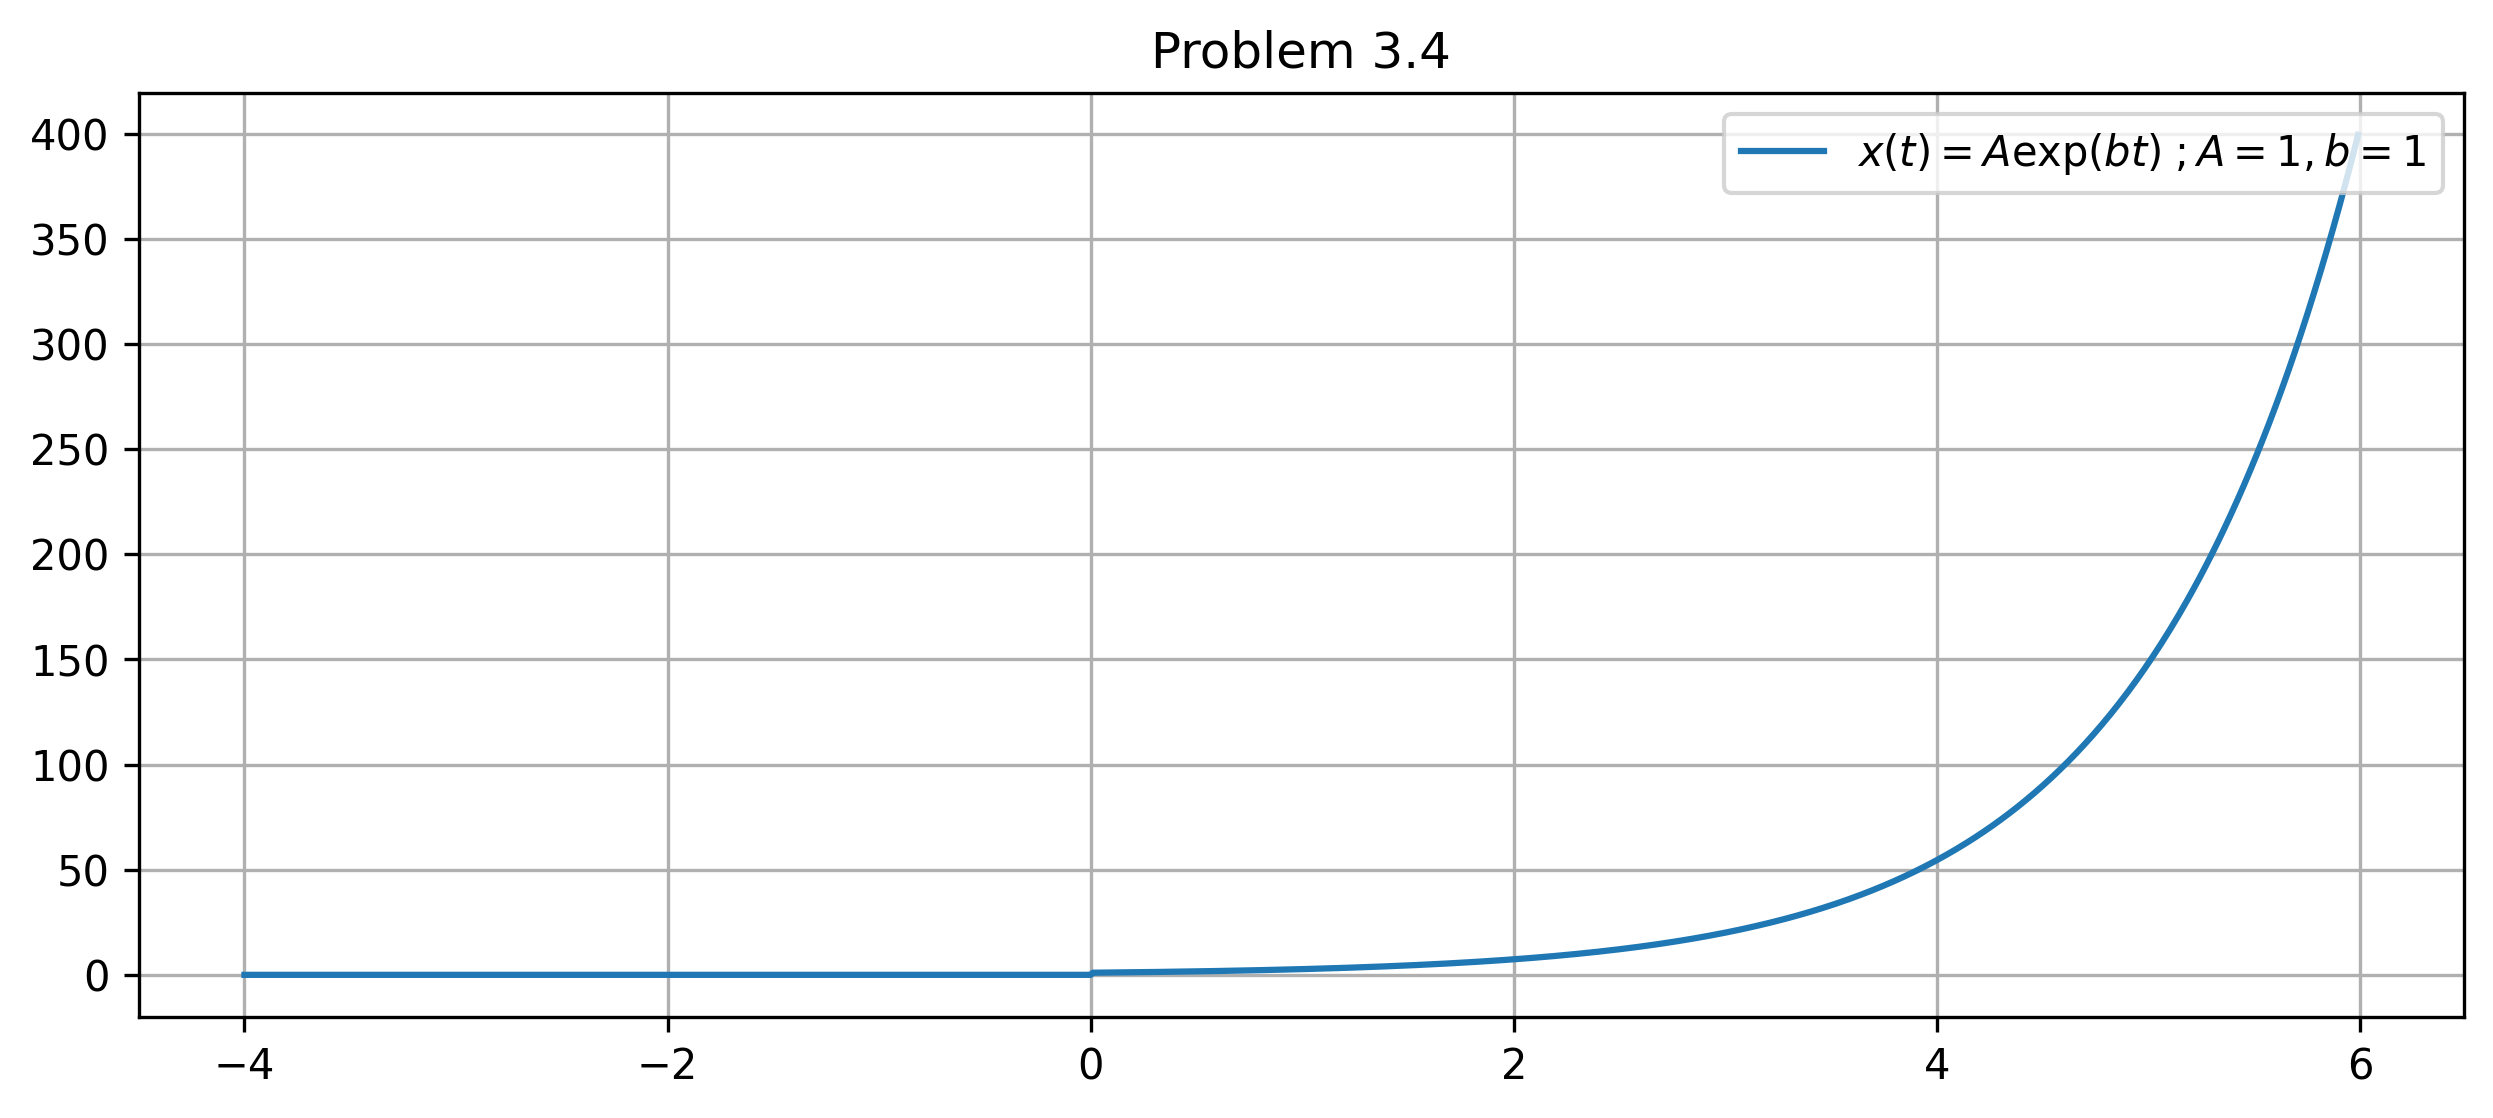
\includegraphics[width=0.8\textwidth]{images/problem_3_4.png}
\end{center}
\end{solution}
% ==================== %
% ================================================================================ %


% ================================================================================ %
%                                    Problem 04                                    %
% ================================================================================ %
\begin{problem}
For the discrete time signal \( x[n] \) shown in Figure below, sketch each of the following

\begin{codingbox}
import matplotlib.pyplot as plt
import numpy as np

fig = plt.figure(figsize=(6, 4))

t = np.arange(-2, 4)
x_t = np.array([-3, 1, 2, -2, 3, -1])

plt.stem(t, x_t)
plt.title('x[n]')
plt.show()
\end{codingbox}

With the resulting plot shown below:
\begin{center}
    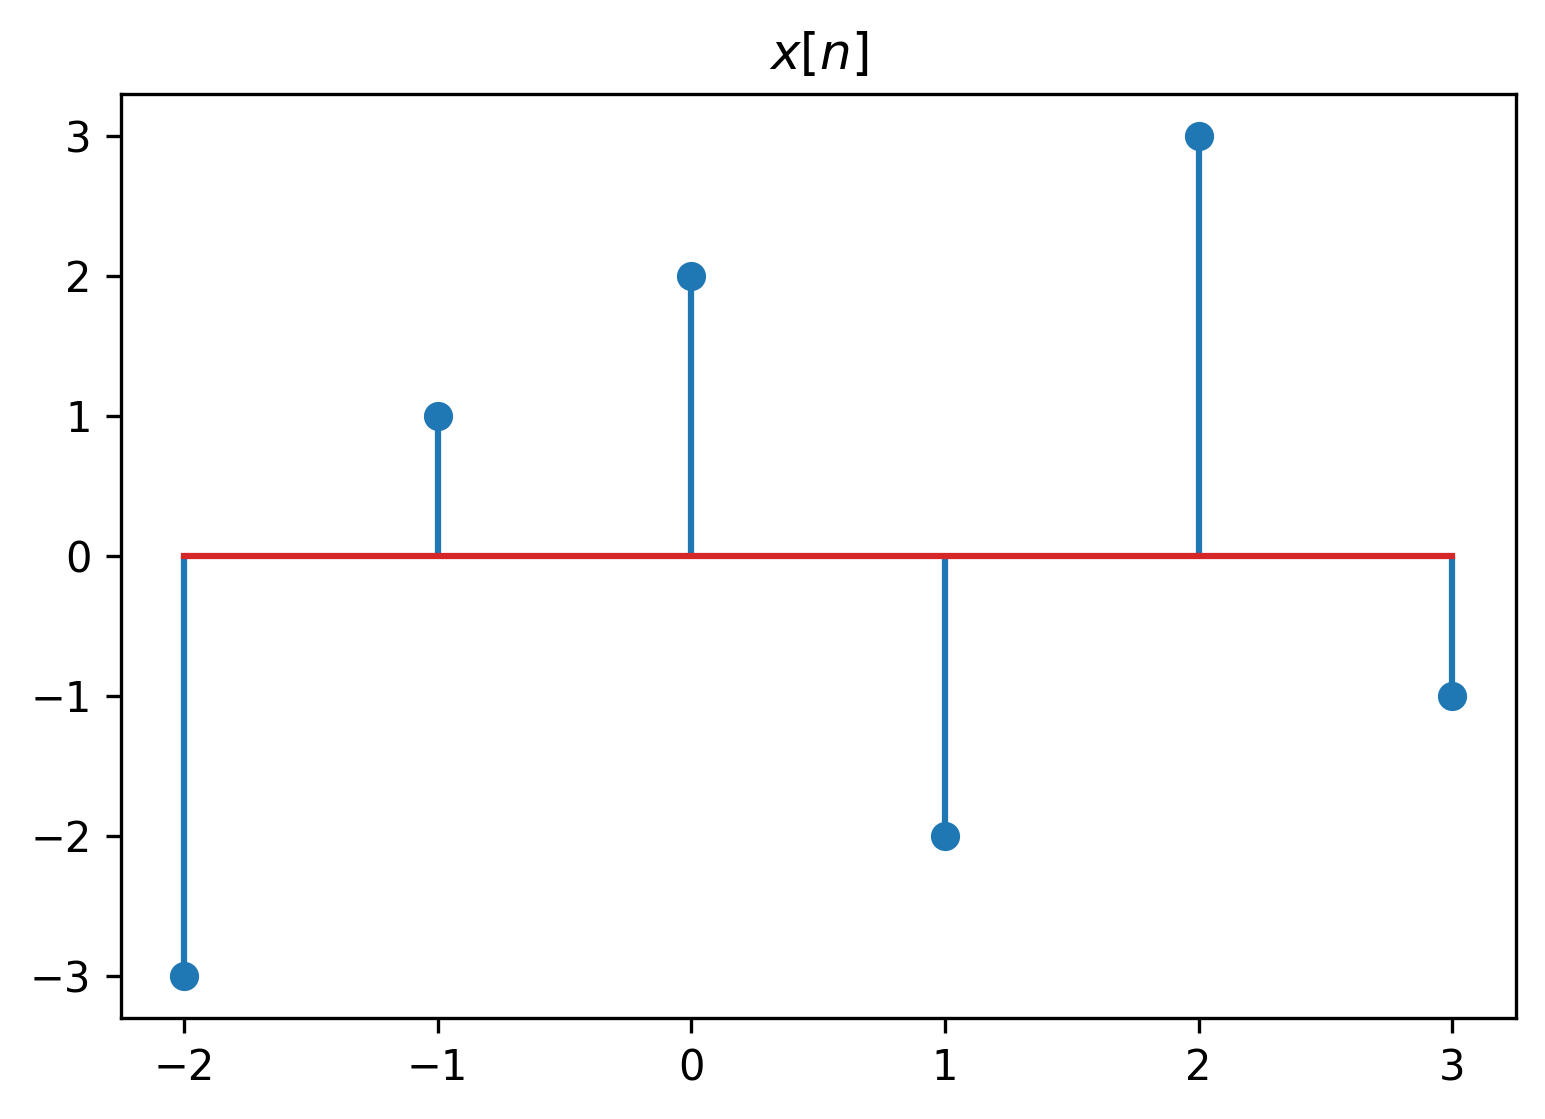
\includegraphics[width=0.5\textwidth]{images/problem_4_xn.png}
\end{center}
\end{problem}

\newpage

\begin{solution}
By using Python, we can create a function to transform the signal based on the given transformation function:
\begin{codingbox}
def transform_signal(x, n, f):
    """Return x[f(n)] for any discrete-time signal x[n]."""
    f_n = f(n)
    f_n_int = f_n[np.floor(f_n) == f_n]
    
    x_new = np.zeros(f_n_int.shape[0], dtype=float)
    
    idx = 0
    for i, val in enumerate(f_n):
        if int(val) == val:
            x_new[idx] = x[i]
            idx += 1
    
    return x_new, f_n_int
\end{codingbox}
\end{solution}

% === Problem 4.1. === %
\begin{tosubmit}
\begin{subproblems}
    \item \( x[2-n] \)
\end{subproblems}

\par\noindent\submitsolution
Using Python and Matplotlib to plot the signal \( x[2-n] \):
\begin{codingbox}
import matplotlib.pyplot as plt
import numpy as np

fig = plt.figure(figsize=(6, 4))

t = np.arange(-2, 4)
x_t = np.array([-3, 1, 2, -2, 3, -1])

x_t, t = transform_signal(x_t, t, lambda x: 2 - x)

plt.stem(t, x_t)
plt.title("x[2 - n]")
plt.show()
\end{codingbox}

With the resulting plot shown below:
\begin{center}
    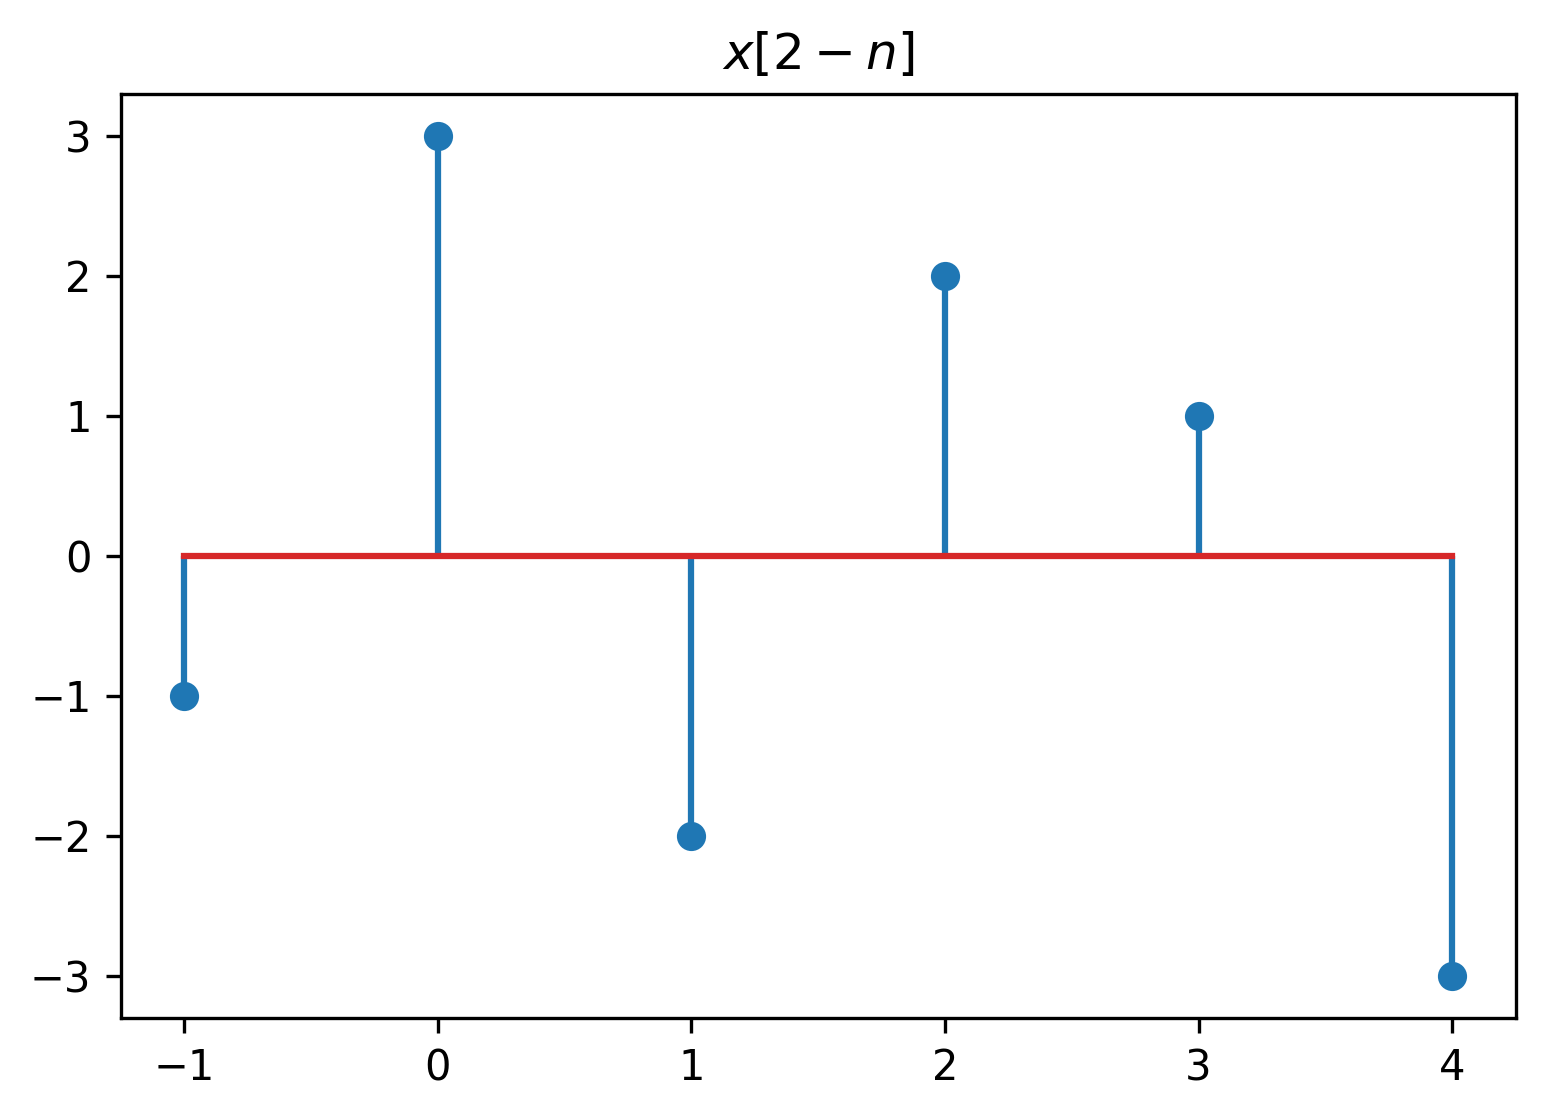
\includegraphics[width=0.5\textwidth]{images/problem_4_1.png}
\end{center}
\end{tosubmit}
% ==================== %

\newpage

% === Problem 4.2. === %
\begin{subproblems}[start=2]
    \item \( x[3n-4] \)
\end{subproblems}

\begin{solution}
Using Python and Matplotlib to plot the signal \( x[3n-4] \):
\begin{codingbox}
import matplotlib.pyplot as plt
import numpy as np

fig = plt.figure(figsize=(6, 4))

t = np.arange(-2, 4)
x_t = np.array([-3, 1, 2, -2, 3, -1])

x_t, t = transform_signal(x_t, t, lambda x: (x + 4) / 3)

plt.stem(t, x_t)
plt.title("x[3n - 4]")
plt.show()
\end{codingbox}

With the resulting plot shown below:
\begin{center}
    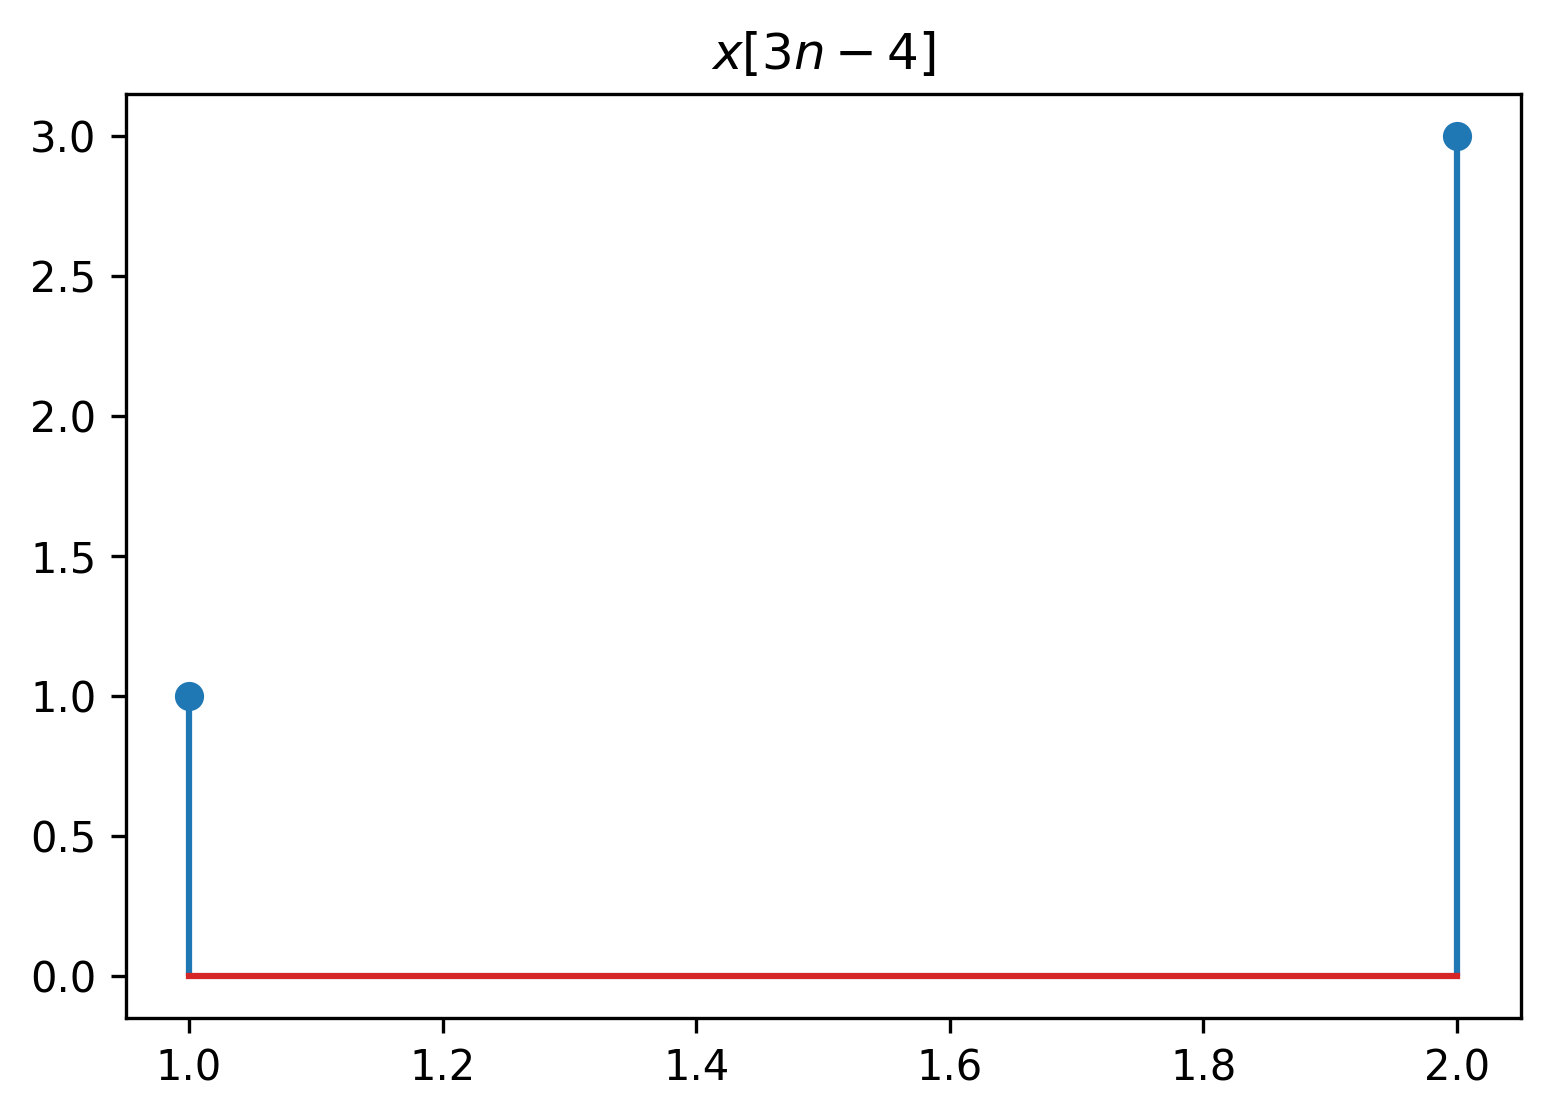
\includegraphics[width=0.5\textwidth]{images/problem_4_2.png}
\end{center}
\end{solution}
% ==================== %


% === Problem 4.3. === %
\begin{tosubmit}
\begin{subproblems}[start=3]
    \item \( x\sqbracket{\frac{2}{3}n+1} \)
\end{subproblems}

\par\noindent\submitsolution
Using Python and Matplotlib to plot the signal \( x[\frac{2}{3}n+1] \):
\begin{codingbox}
import matplotlib.pyplot as plt
import numpy as np

fig = plt.figure(figsize=(6, 4))

t = np.arange(-2, 4)
x_t = np.array([-3, 1, 2, -2, 3, -1])

x_t, t = transform_signal(x_t, t, lambda x: (x - 1) * 3 / 2)

plt.stem(t, x_t)
plt.title("x[(2/3)n + 1]")
plt.show()
\end{codingbox}

\newpage

With the resulting plot shown below:
\begin{center}
    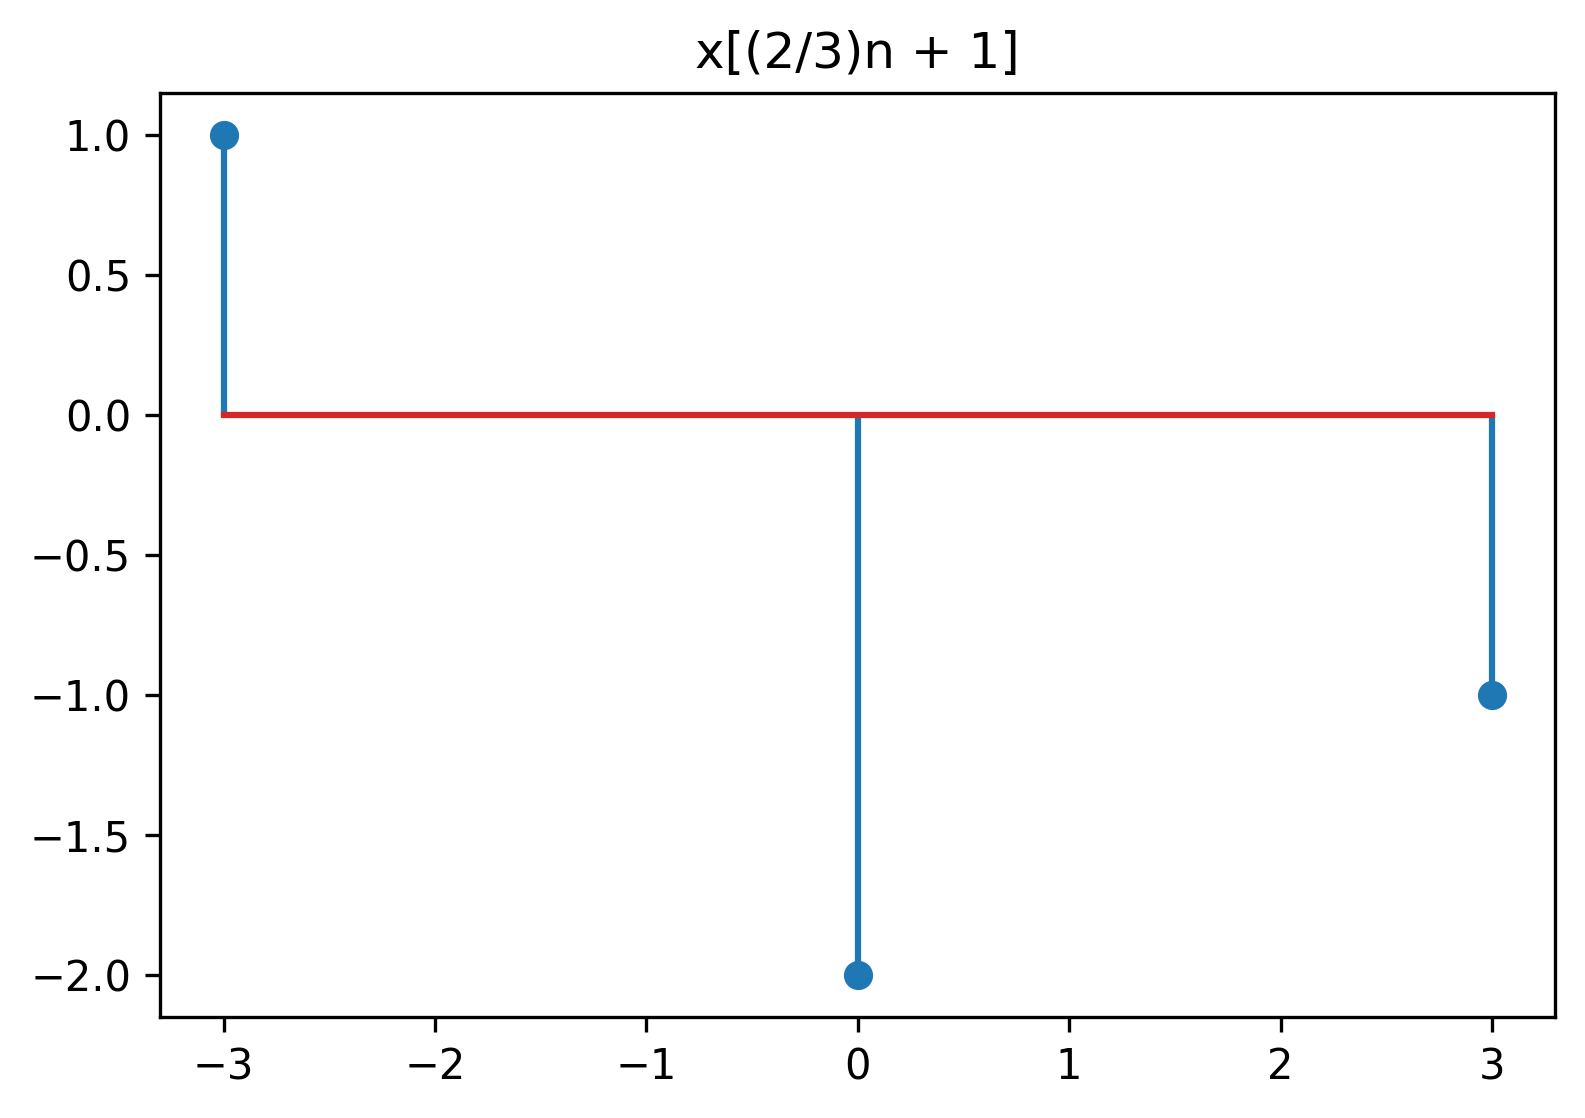
\includegraphics[width=0.5\textwidth]{images/problem_4_3.png}
\end{center}
\end{tosubmit}
% ==================== %


% === Problem 4.4. === %
\begin{subproblems}[start=4]
    \item \( x\sqbracket{-\frac{n+8}{4}} \)
\end{subproblems}

\begin{solution}
Using Python and Matplotlib to plot the signal \( x\sqbracket{-\frac{n+8}{4}} \):
\begin{codingbox}
import matplotlib.pyplot as plt
import numpy as np

fig = plt.figure(figsize=(6, 4))

t = np.arange(-2, 4)
x_t = np.array([-3, 1, 2, -2, 3, -1])

x_t, t = transform_signal(x_t, t, lambda x: (-4 * x) - 8)

plt.stem(t, x_t)
plt.title("x[-(n + 8) / 4]")
plt.show()
\end{codingbox}

With the resulting plot shown below:
\begin{center}
    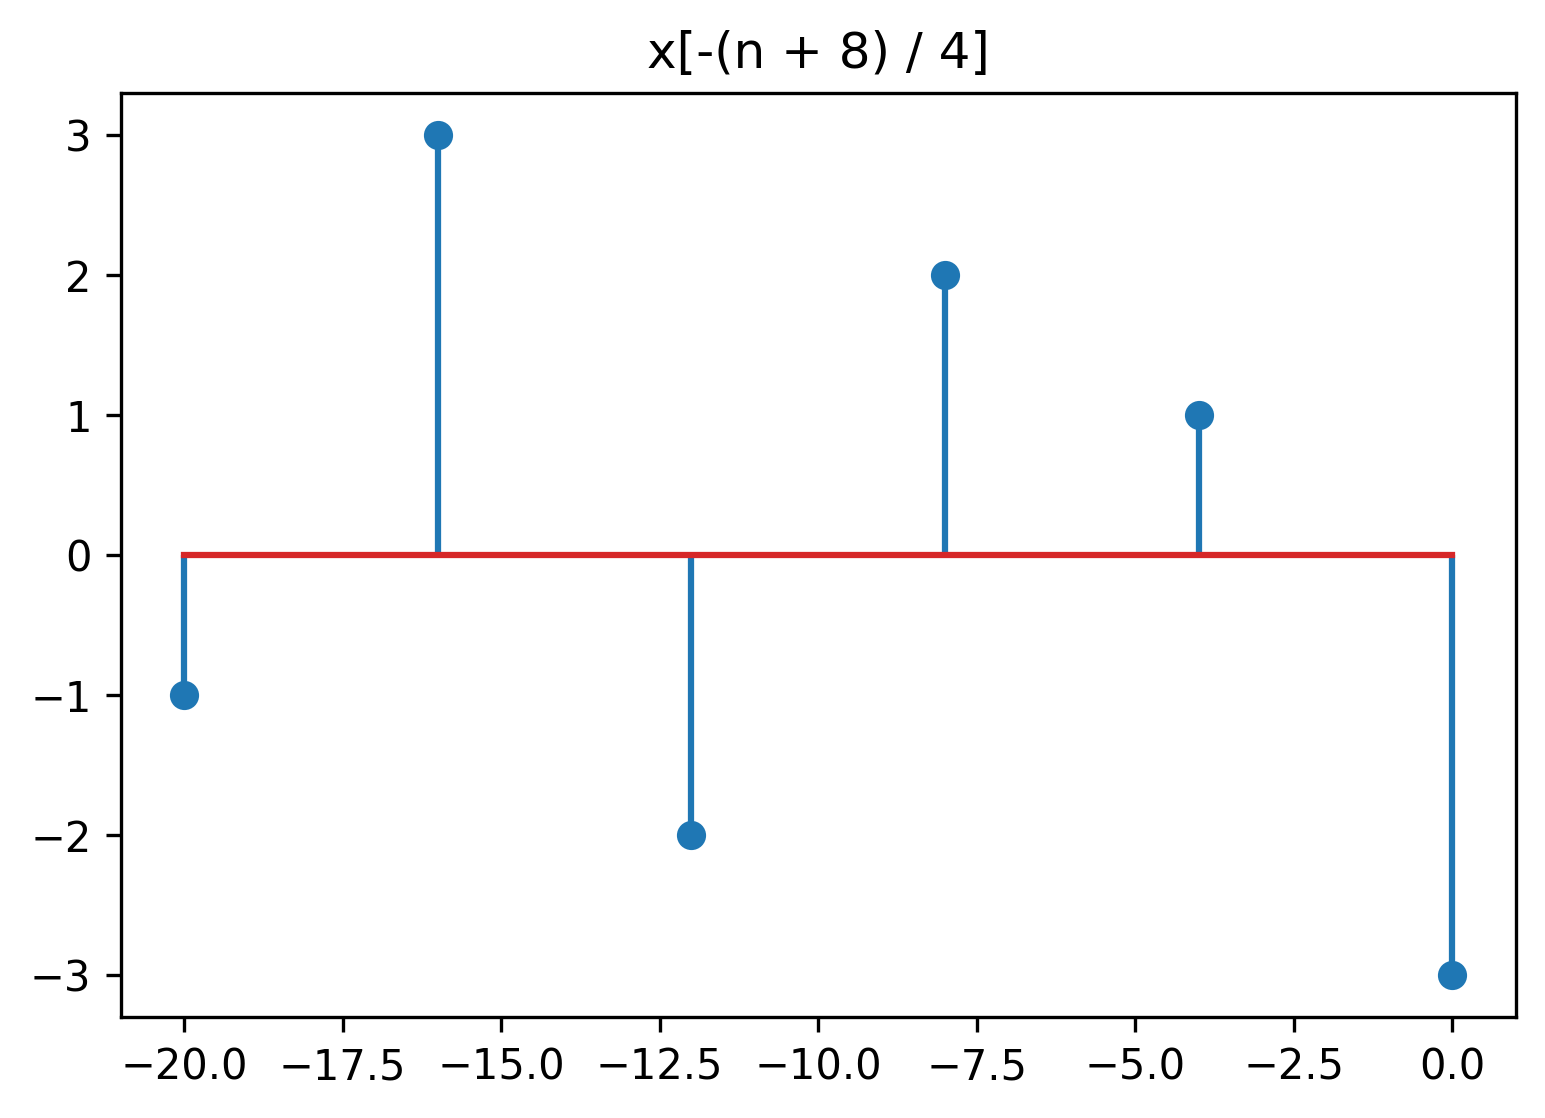
\includegraphics[width=0.5\textwidth]{images/problem_4_4.png}
\end{center}
\end{solution}
% ==================== %

\newpage

% === Problem 4.5. === %
\begin{tosubmit}
\begin{subproblems}[start=5]
    \item \( x[n^3] \)
\end{subproblems}

\par\noindent\submitsolution
Using Python and Matplotlib to plot the signal \( x[n^3] \):
\begin{codingbox}
import matplotlib.pyplot as plt
import numpy as np

fig = plt.figure(figsize=(6, 4))

t = np.arange(-2, 4)
x_t = np.array([-3, 1, 2, -2, 3, -1])

x_t, t = transform_signal(x_t, t, lambda x: np.cbrt(x))

plt.stem(t, x_t)
plt.title("x[n^3]")
plt.show()
\end{codingbox}

With the resulting plot shown below:
\begin{center}
    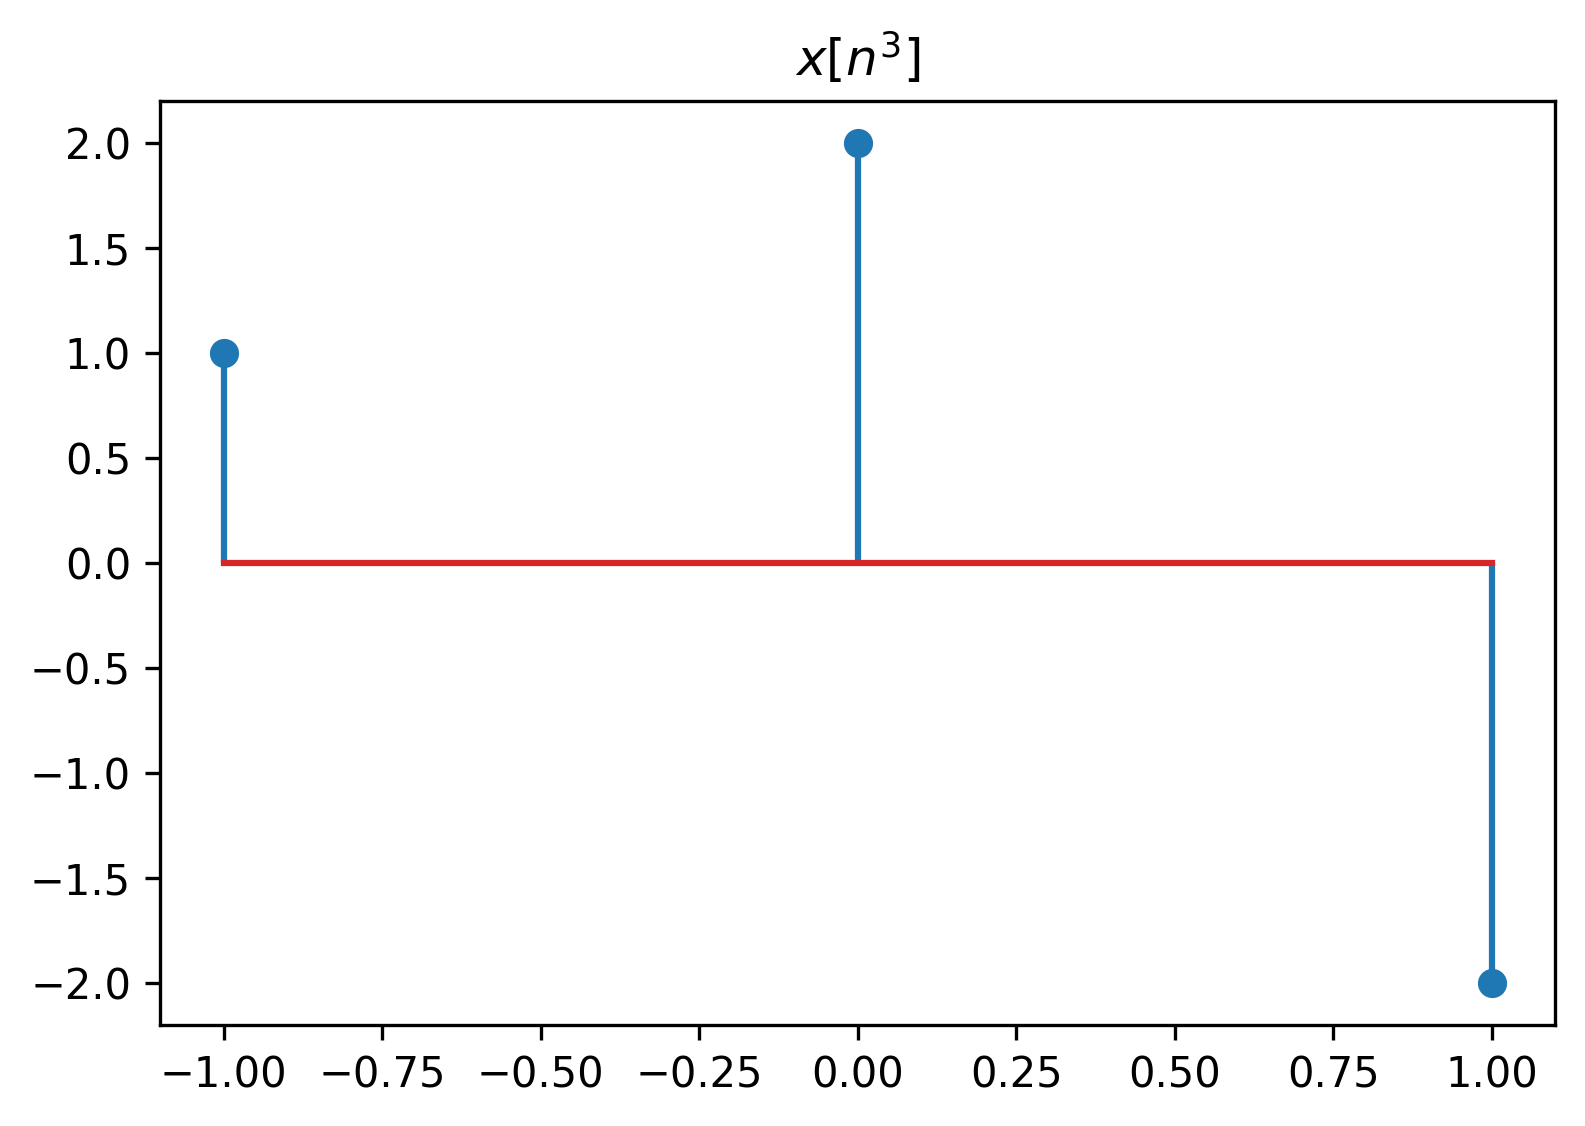
\includegraphics[width=0.5\textwidth]{images/problem_4_5.png}
\end{center}
\end{tosubmit}
% ==================== %


% === Problem 4.6. === %
\begin{subproblems}[start=6]
    \item \( x[2-n] + x[3n-4] \)
\end{subproblems}

\begin{solution}
Introduce a helper function to add two signals:
\begin{codingbox}
def add_discrete_signals(x1, t1, x2, t2):
    """Return x1[n] + x2[n] for any discrete-time signals x1[n] and x2[n]."""
    t = np.union1d(t1, t2)
    x = np.zeros(t.shape[0], dtype=float)
    
    for i, val in enumerate(t):
        if val in t1:
            x[i] += x1[np.where(t1 == val)[0][0]]
        if val in t2:
            x[i] += x2[np.where(t2 == val)[0][0]]
    
    return x, t
\end{codingbox}

\newpage

Using Python and Matplotlib to plot the signal \( x[n^3] \):
\begin{codingbox}
import matplotlib.pyplot as plt
import numpy as np

fig = plt.figure(figsize=(6, 4))

t = np.arange(-2, 4)
x_t = np.array([-3, 1, 2, -2, 3, -1])

x_t_1, t_1 = transform_signal(x_t, t, lambda x: 2 - x)
x_t_2, t_2 = transform_signal(x_t, t, lambda x: (x + 4) / 3)

x_t, t = add_discrete_signals(x_t_1, t_1, x_t_2, t_2)

plt.stem(t, x_t)
plt.title("x[2-n] + x[3n-4]")
plt.show()
\end{codingbox}

With the resulting plot shown below:
\begin{center}
    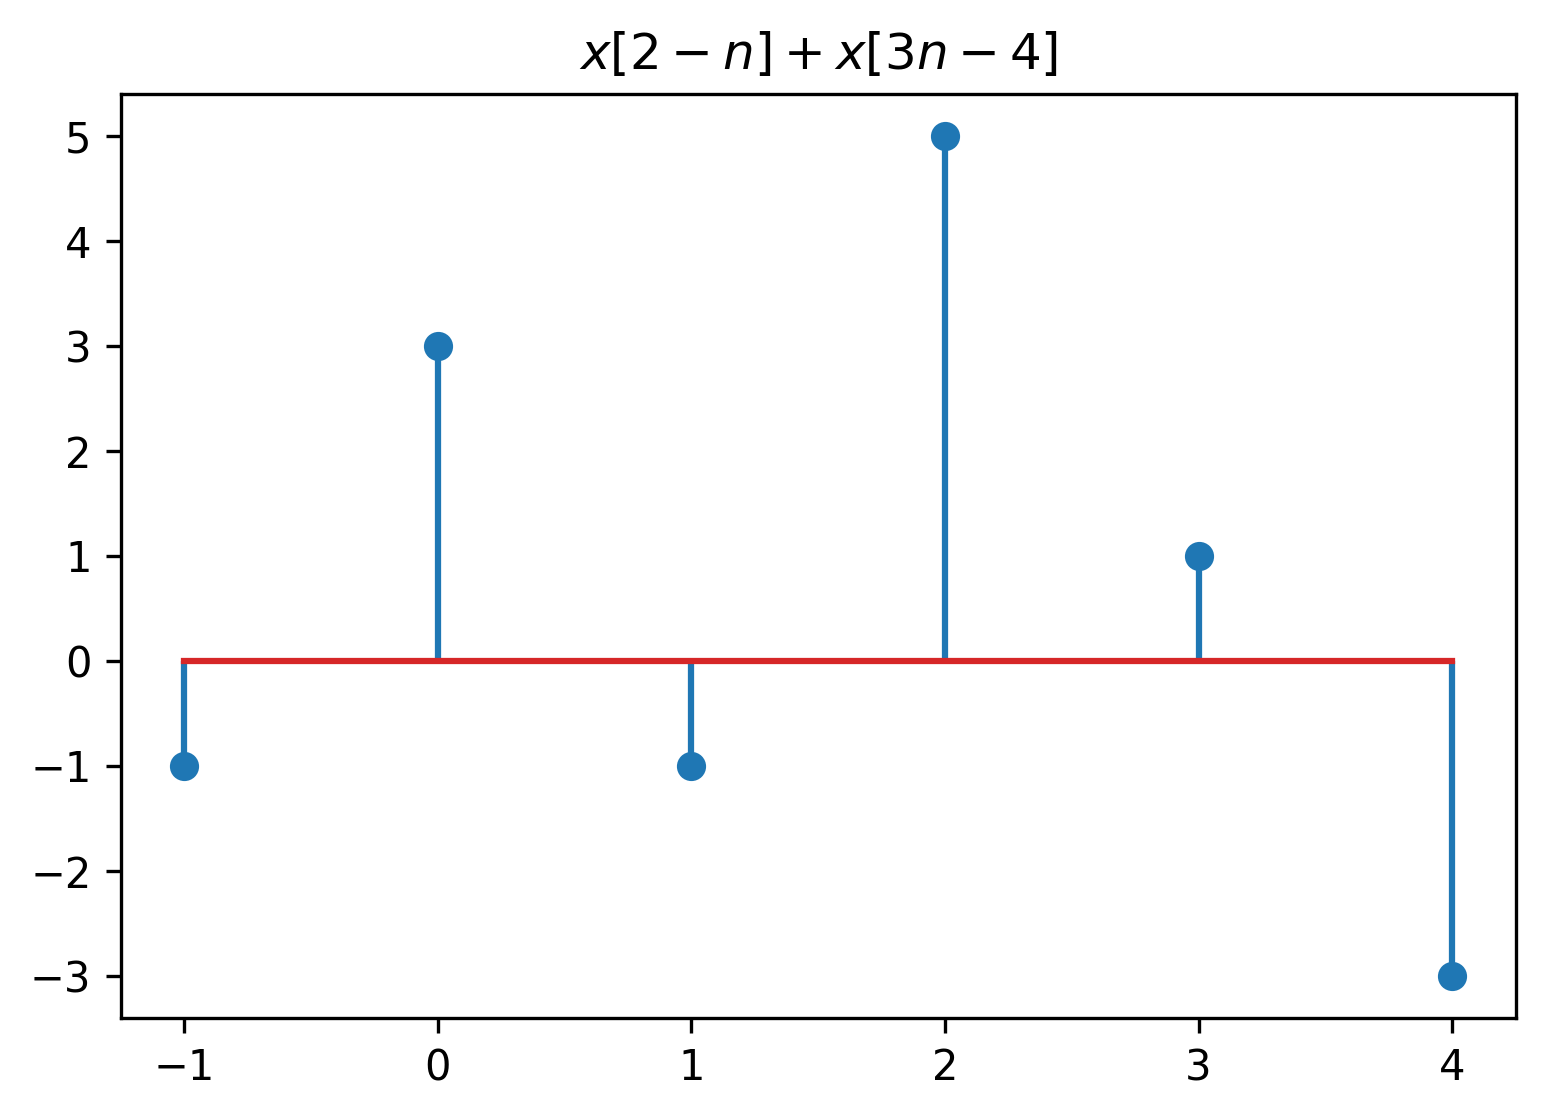
\includegraphics[width=0.5\textwidth]{images/problem_4_6.png}
\end{center}
\end{solution}
% ==================== %
% ================================================================================ %


\end{document}